\documentclass[ngerman,a4paper,oneside,titlepage, openright, 10pt]{report}
\usepackage[ngerman]{babel}
%\usepackage[ansinew]{inputenc}
\usepackage[ansinew]{inputenc}
\usepackage[numbers,square]{natbib}
%\documentclass[ngerman]{scrartcl}
\usepackage{graphicx}
\usepackage{fancyhdr}
\usepackage{capt-of}
\usepackage{setspace}
\usepackage[font=bf]{caption}
\usepackage{chngcntr}
%\usepackage[hidelinks=true]{hyperref}
\usepackage[pdfborder={0 0 0}]{hyperref}
\usepackage{listings}
\usepackage{color}
\usepackage{amsmath}
\usepackage[T1]{fontenc}
\usepackage[bottom=4cm]{geometry}
\usepackage{booktabs}
\usepackage{natbib}
\usepackage{hyphenat}
\usepackage{float}

%\usepackage[automark]{scrpage2}
\newcommand{\changefont}[3]{\fontfamily{#1} \fontseries{#2} \fontshape{#3} \selectfont}
\normalfont

%\DeclareCaptionFont{white}{\color{white}}
\DeclareCaptionFormat{listing}{\colorbox{white}{\parbox{\textwidth}{#1#2#3}}}
%\captionsetup[lstlisting]{format=listing,labelfont=black,textfont=white}
\definecolor{dkgreen}{rgb}{0.0,0.55,0}
\definecolor{gray}{rgb}{0.95,0.95,0.95}
\definecolor{mauve}{rgb}{0.58,0,0.82}


\lstset{
  language=C++,                % choose the language of the code
  basicstyle=\scriptsize\ttfamily, % fontsize \tiny \scriptsize \small
  numbers=left,                   % where to put the line-numbers
  stepnumber=1,                   % the step between two line-numbers.        
  numbersep=4pt,                  % how far the line-numbers are from the code
  backgroundcolor=\color{gray},   % choose the background color. You must add \usepackage{color}
  showspaces=false,               % show spaces adding particular underscores
  showstringspaces=false,         % underline spaces within strings
  showtabs=false,                 % show tabs within strings adding particular underscores
  tabsize=2,                      % sets default tabsize to 2 spaces
  captionpos=t,                   % sets the caption-position to bottom
  breaklines=false,               % sets automatic line breaking
  breakatwhitespace=true,         % sets if automatic breaks should only happen at whitespace
  xleftmargin=4pt,
 % title=\lstname,                % show the filename of files included with \lstinputlisting;
  keywordstyle=\color{blue},      % keyword style
  commentstyle=\color{dkgreen},   % comment style
  stringstyle=\color{mauve},      % string literal style
}


\counterwithin{figure}{chapter}
\onehalfspacing
\setlength{\headheight}{15pt}

\newcommand{\blankpage}{
\newpage
\thispagestyle{empty}
\mbox{}
\newpage
}
 
 \raggedbottom
\begin{document}


\changefont{ptm}{m}{n}
%\fontfamily{ptm}\fontseries{m} \fontshape{n} \selectfont
\nocite{*}
\bibliographystyle{plain}
\renewcommand{\thepage}{\Roman{page}}
\setcounter{secnumdepth}{-2}

\thispagestyle{empty}
\begin{titlepage}
	\begin{flushleft}
			Bauhaus-Universit�t Weimar\\
			Fakult�t Medien\\
			Studiengang Mediensysteme
	\end{flushleft}
	\begin{verbatim}


	\end{verbatim}
	\begin{center}
		\Large \textbf{Erstellung, Segmentierung und Out-Of-Core Speichermanagement von Sparse Voxel Octrees}
\begin{figure}[position=h]
  \centering
  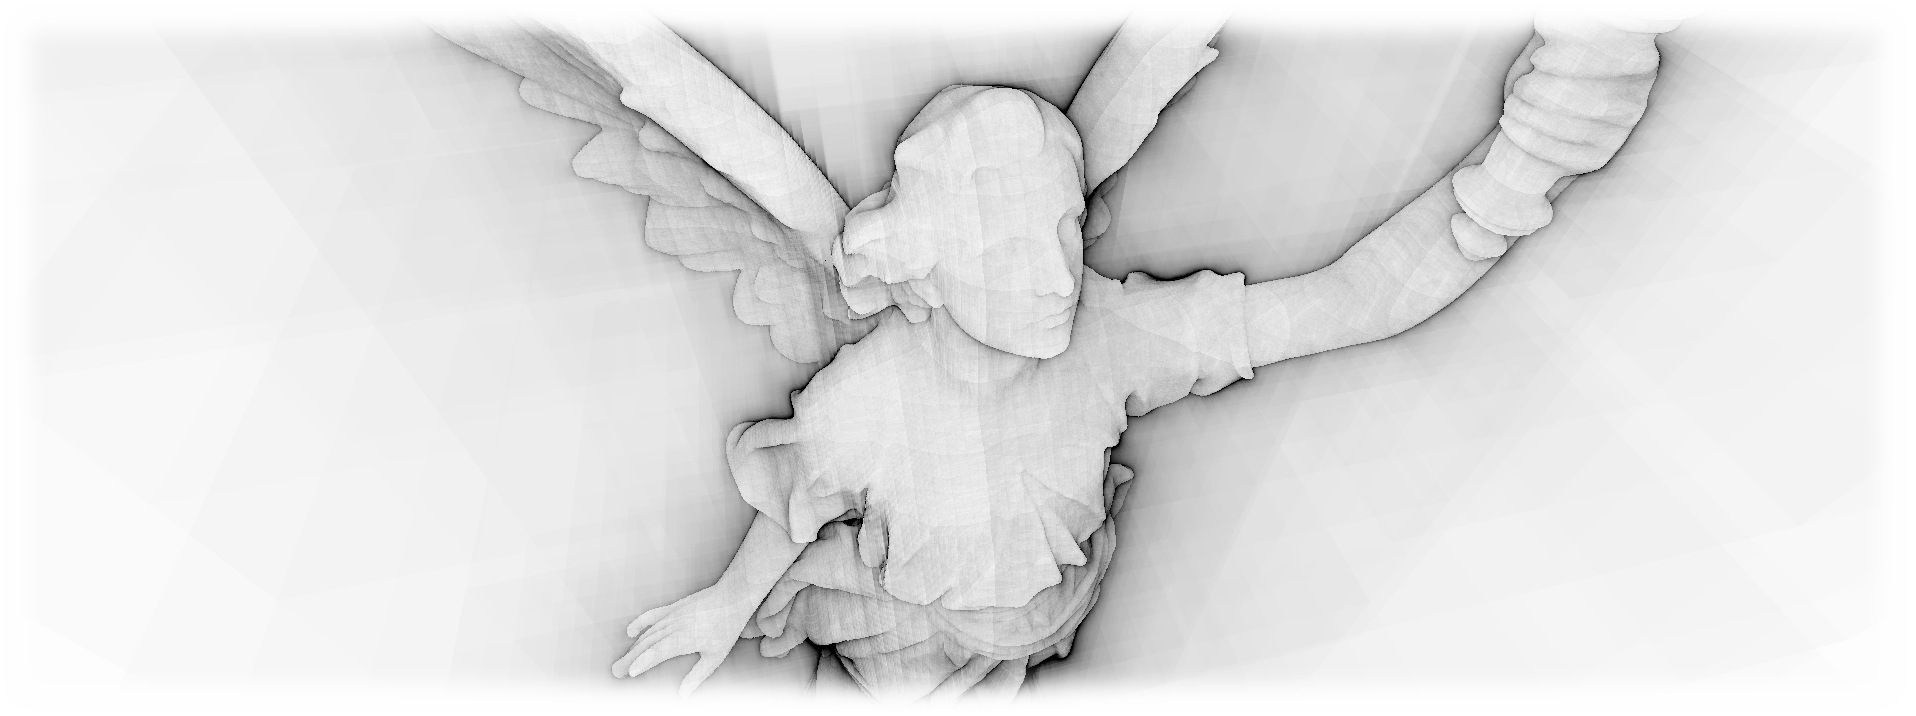
\includegraphics[width=1.0\textwidth]{figures/title_01.png}
\end{figure}

		\Large Diplomarbeit
	\end{center}
	\begin{verbatim}






	\end{verbatim}
	\begin{center}
		Felix Wei�ig\\
		Matrikelnummer: ------\\
		geb. am 10.10.1979 in Hoyerswerda\\
	\begin{verbatim}


	\end{verbatim}
		1. Gutachter: Prof. Dr. Charles A. W�thrich\\
		%2. Gutachter: Prof. Dr. Guido Morgenthal \,\,\,


	\begin{verbatim}

	\end{verbatim}
	Datum der Abgabe: 25. M�rz 2013
	\end{center}

	
\end{titlepage}

\section{Erkl�rung}

Hiermit versichere ich, dass ich die vorliegende Diplomarbeit selbstst�ndig angefertigt, 
anderweitig nicht f�r Pr�fungszwecke vorgelegt und alle verwendeten Quellen angegeben habe.
\begin{verbatim}




\end{verbatim}
Felix Wei�ig
\begin{verbatim}



\end{verbatim}
Weimar, den 25. M�rz 2013

\blankpage
\section{Danksagung}
An dieser Stelle m�chte ich mich zun�chst bei Prof. Dr. Charles W�thrich f�r die Annahme und Bewertung meiner Diplomarbeit bedanken. Ein Dank geht auch an Bernhard Bittorf, dessen moralische Unterst�tzung mir w�hrend des Entstehens der Arbeit sehr geholfen hat. Ein gro�er Dank geht vor allem an Henning Gr�ndl, Sebastian Thiele, Konstantin Silin und Stephan Beck f�r lebhafte Diskussionen und Hilfe bei der Bearbeitung des schriftlichen Teils dieser Arbeit. Benjamin Bendig muss im Besonderen f�r seine hervorragende Arbeit bei der Implementation des in dieser Arbeit verwendeten OpenCL-Wrappers \textit{benCL} erw�hnt werden. Kaum genug danken kann ich meinen Eltern f�r die jahrelange Unterst�tzung w�hrend meines ausschweifenden Studiums.\\
Der gr��te Dank geht jedoch an meine Freundin und Lebensgef�hrtin Eva Johanna M�hlemann, die mir in den zur�ckliegenden Monaten den R�cken frei hielt und mir dadurch den Freiraum gab diese Arbeit zu bew�ltigen.

Danke.  

\blankpage
\section{Kurzfassung}

Voxel+Ray=Pixel
\addtocontents{toc}{\protect\thispagestyle{empty}}
\tableofcontents
\thispagestyle{empty}
\listoffigures
\blankpage
\thispagestyle{empty}
\renewcommand{\thepage}{\arabic{page}}
\setcounter{secnumdepth}{2}


%\pagestyle{scrheadings} 
%\clearscrheadfoot 
%\ihead{\headmark} 
%\ohead{Name} 
%\renewcommand*{\chapterpagestyle}{chapter}

\newpage
\renewcommand{\sectionmark}[1]{}
\setcounter{page}{1}

\fancyhf{} % clear all header and footer fields
%\fancyfoot[C]{\thepage} % except the center
%\fancyhead[EL]{\nouppercase{\leftmark}}
%\fancyhead[OL]{\nouppercase{\rightmark}}


\fancyfoot[LE,RO]{\thepage}
\pagestyle{fancy}
\fancyhead[LE,RO]{\slshape \rightmark}
\fancyhead[LO,RE]{\slshape \leftmark}
%\renewcommand{\chaptermark}[1]{\markboth{\thechapter.\space#1}{}}

\renewcommand{\chaptermark}[1]{\markright{#1}{}}
  \makeatletter
 \let\ps@plain\ps@fancy
 \makeatother
\chapter{Einleitung}
\section{Motivation}
Seit langer Zeit ist die Bild\-synthese durch Ras\-teris\-ierung von pa\-rame\-tri\-sierten Dreiecken der Quasi-Standard f�r Echtzeitcomputergrafik. Diese Entwicklung wurde nicht zuletzt durch die Einf�hrung von dedizierter Hardware und offenen Standards, wie OpenGL m�glich. Der Vorteil von Dreiecken als Geometrieprimitiv ist, dass sich mit ihnen sehr effizient planare Fl�chen darstellen lassen. Dabei hat die Gr��e der abgebildeten Fl�chen keinen Einfluss auf den Speicherbedarf der Repr�sentation. In modernen Anwendungen wie Spielen oder bei der Darstellung von hochaufl�senden 3D-Scanns ist dieser Vorteil jedoch immer weniger relevant da der �berwiegende Teil des ben�tigten Speichers durch Texturen belegt wird. Diese werden ben�tigt um die Fl�chen mit Details zu versehen, wie Farbe, Richtung und anderen zur Beleuchtung ben�tigten Attributen. Dabei ist die Parametrisierung von komplex geformten Dreiecksnetzen mit Textur\-koordinaten nicht trivial und muss meist von Hand bewerkstelligt werden.\\
Bei der Rasterisierung von detaillierten Dreiecksnetzen mit hochaufgel�sten Texturen kommt es zu Ali\-asing\-artefakten. Um diese zu reduzieren werden von Dreiecks\-netzen und Texturen niedriger aufgel�ste, sta\-tische Versionen erzeugt (\textit{Level-of-Detail, LOD}). Zwischen diesen Versionen wird bei der Darstellung je nach Betrachtungsabstand gewechselt, was zu st�renden \textit{Popping}-Artifakten f�hrt wenn eine LOD-Stufe durch eine andere ausgetauscht wird. Mit dieser Technik kann nur selten ein ideales Verh�ltnis zwischen Geometrie- und Bildaufl�sung gew�hrleistet werden. Dynamische Erzeugung von LOD-Stufen ist mit hohem Rechen- oder Speicheraufwand verbunden. Au�erdem muss das LOD-Problem f�r Geometrie- und Texturdaten w�hrend der Erstellung und der Darstellung separat gel�st werden. Ein Nachteil des Rasterisierungsansatzes ist das Fehlen von globalen Informationen w�hrend der Fragmentgenerierung. Jedes Primitiv wird f�r sich behandelt, ohne dass globale Informationen zur Optimierung (\textit{Culling}) oder Beleuchtung (\textit{Global Illumination}) zur Verf�gung stehen.
\begin{figure}[position=h]
  \centering
  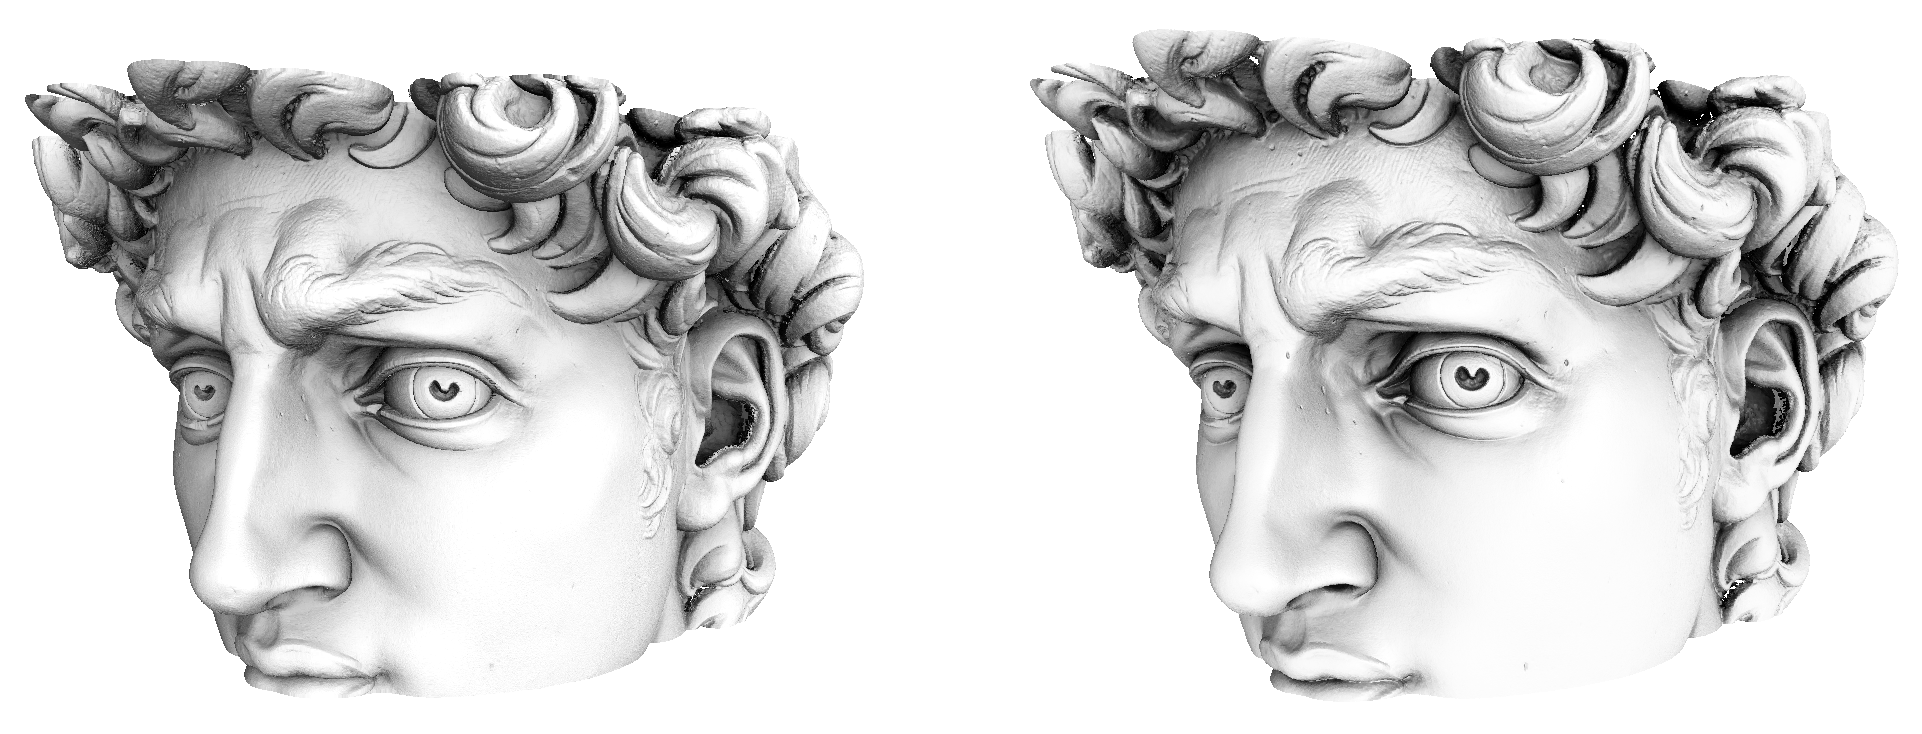
\includegraphics[width=1.0\textwidth]{figures/mesh_and_svo.png}
  \caption{Darstellung von Dreicksnetz und Sparse Voxel Octree \label{mesh_and_svo}}
\end{figure}
Die Generalisierung der Renderpipelines und die Einf�hrung von GPGPU-Hochsprachen wie OpenCL machen es m�glich, die Frage nach geeigneten Geometrieprimitiven und Bildsyntheseverfahren neu zu stellen. Sparse Voxel Octree (SVO) als Datenstruktur in Kombination mit \textit{Raycasting} als Algorithmus zur Bildsynthese bieten viele positive Eigenschaften. Sparse Voxel Octrees vereinen Geometrie- und Texturdaten in einer gemeinsamen hierarchischen Datenstruktur. Durch Raycasting auf dieser Struktur kann das LOD-Problem f�r Geometrie- und Texturdaten gleichzeitig pro Bildpunkt gel�st werden. Der Octree wirkt dabei als eine Beschleunigungs\-struktur, so dass w�hrend des Traversierens nur die Teile der Struktur durchlaufen werden, die zur Bildsynthese beitragen. Eine Parametrisierung ist nicht notwendig da jedes Voxel seine ei\-genen Attributinformationen spei\-chert die f�r seine Gr��e in optimaler Aufl�sung vorliegen. Abbildung \ref{mesh_and_svo} zeigt die Darstellung eines Modells als Dreiecksnetz (linkes Bild) und als Sparse Voxel Octree (rechtes Bild).\\
Dennoch gibt es einige Herausforderungen die vor der Verwendung von Sparse Voxe Octrees bew�ltigt werden m�ssen. Sparse Voxel Octrees ben�tigen viel Speicher. Die Menge an Arbeitsspeicher aktueller Grafikkarten ist f�r einige Anwendungen ausreichend, um SVO-Strukturen in hinreichend hoher Aufl�sung zu speichern. Ben�tigt man jedoch h�here Aufl�sung, um m�glichst viele Details beziehungsweise sehr gro�e Strukturen abbilden zu k�nnen, fallen schnell mehrere Gigabyte an Daten an, die dann nicht mehr als Ganzes in den GPU-Speicher passen.
Da Sparse Voxel Octrees erst in j�ngster Zeit in den Fokus von Wissenschaft und Industrie ger�ckt sind, sind sie in Programmen zur Erstellung von 3D-Inhalten noch nicht angekommen. Daher ist es zun�chst notwendig Sparse Voxel Octrees aus anderen Geometrie\-repr�sentationen zu erstellen. Dreicksnetze, Punktwolken, H�henfelder oder Volumendaten k�nnen als Eingabedaten dienen. Um unterschiedliche Repr�sentationen von Inhalten ohne gro�en Ent\-wicklungs\-aufwand unterst�tzen zu k�nnen fehlt ein generisches System das diese Daten verarbeiten kann.


\section{Zielstellung}
Ziel dieser Arbeit soll die Entwicklung eines Out-Of-Core Ansatzes sein, der basierend auf Segmentierung der Daten eine adaptive Verfeinerung der Darstellung erm�glicht. Um dies zu unterst�tzen soll au�erdem ein generisches Systems zur Erstellung von SVO-Strukturen aus unterschiedlichen Eingabedaten wie Dreiecksnetzen, Punktwolken oder Volumendaten entwickelt werden. Die Bildgenerierung soll durch Raycasting auf den erzeugten Sparse-Voxel-Octree-Strukturen erm�glicht werden. Die n�tigen Berechnungen sollen auf aktueller Grafik-Hardware ausgef�hrt werden um interaktive Bild\-wiederhol\-raten zu erreichen.



\blankpage
\chapter{Repr�sentation und Verwendung von Volumendaten in der Computergrafik}


\section{Volumendaten}

Volumendaten k�nnen durch dreidimensionale, �quidistante Gitter beschrieben werden. Die Kreuzungspunkte der Gitter werden \textit Voxel (Volumen-Pixel) genannt. Jeder Voxel kann einen einzelnen skalaren Wert, wie beispielsweise Dichte oder Druck, oder mehrere skalare Werte wie Farben und Richtungsinformationen enthalten. Dadurch eignet sich diese Darstellung zur Repr�sentation eines �quidistant gesampelten Raumes, der nicht homogen gef�llt ist. Durch die uniforme Unterteilung des Raumes ist die Position und die Ausdehnung eines jeden Voxels implizit in der Datenstruktur enthalten und muss daher nicht gespeichert werden.
\begin{figure}[position=h]
  \centering
  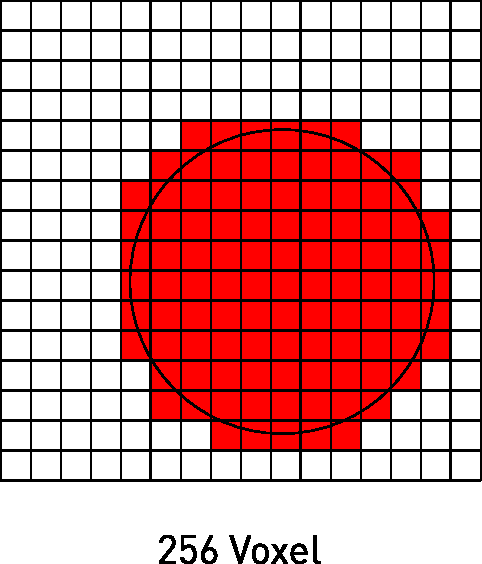
\includegraphics[width=0.32\textwidth]{figures/cut_volume.pdf}
  \caption{Schnitt durch ein Volumen Gitter \label{cut_volume}}
\end{figure}
Volumendaten werden vorwiegend in der Medizin, beispielsweise als Ausgabe der Magnet\-resonanz\-tomographie oder in der Geologie zum Abbilden der Ergebnisse von Reflexions\-seismik\-verfahren verwendet.\\
Um eine hinreichende Aufl�sung der Volumenrepr�sentation zu gew�hrleisten sind gro�e Datenmengen erforderlich. Ein mit $512^3$ Voxeln aufgel�stes Volumen, dessen Voxel jeweils einen mit 4 Byte abgebildeten Skalar enthalten, belegt bereits 512 Megabyte. Verdoppelt man die Aufl�sung auf $1024^3$, verachtfacht sich der Speicherbedarf auf 4 Gigabyte. Volumendaten enthalten in der Regel einen gro�en Anteil an homogenen Bereichen die durch ein regul�res Gitter als viele Einzelwerte abgebildet werden m�ssen. Daher gibt es Datenstrukturen die ausgehend von dem regul�ren Gitter eine hierarchische Struktur erzeugen, um diese Bereiche zusammenzufassen.



%  ////////////////////////////////////////////////////////////////////


\subsection{Octrees}
Ein Octree ist eine raumteilende, rekursive Datenstruktur. Ein initiales, kubisches Volumen wird in acht gleich gro�e Untervolumen geteilt. Die Teilung wird f�r jedes Untervolumen fortgef�hrt, bis eine maximale Tiefe beziehungs\-weise ein maximaler Unterteilungsgrad erreicht ist. Mit jeder Tiefen\-stufe des Octrees verdoppelt sich die Aufl�sung der abbildbaren Information auf jeder Achse. Die Gr��e eines Voxels kann mit $ 2^{-d} $ bestimmt werden wobei $d$ die Tiefe des Voxels in der Baumstruktur, beginnend mit $d=0$ f�r die Wurzel, ist. F�r vollbesetzte Octrees l�sst eine Darstellung im Speicher aus der Struktur ableiten. Da jeder Elternknoten genau acht Kinder besitzt, kann innerhalb einer seriellen Struktur implizit auf seine Kind\-knoten geschlossen werden. Die Positionen der Kinder eines Knotens kann durch die Funktion $ C(P,n) = 8*P+n $ berechnet werden wobei $P$ der Index des Elternknotens, $n$ die Nummer des Kindes (beginnend mit 1) und das resultierende $C$ der Index des Kindknotens ist.\\
\\
Bereiche in Volumendaten, die homogene Daten enthalten oder leer sind,k�nnen jedoch von der Unterteilung ausgeschlossen werden, wodurch eine wesentlich kompaktere Darstellung der Daten gegen�ber konventionellen Volumendaten erreicht werden kann. Daf�r muss f�r jedes Voxel ein Verweis auf die ihn unterteilenden Untervolumen existieren. In der Regel besitzt jedes Voxel eines solchen Octrees acht Kinder (\textit{innerer Knoten}) oder kein Kind (\textit{Blatt-Knoten}). Die im ung�nstigsten Fall zu speichernden sieben leeren Knoten sind bei dieser Darstellung n�tig um homogene Bereiche innerhalb des Eltern-Voxels zu kodieren.
\begin{figure}[position=h]
  \centering
  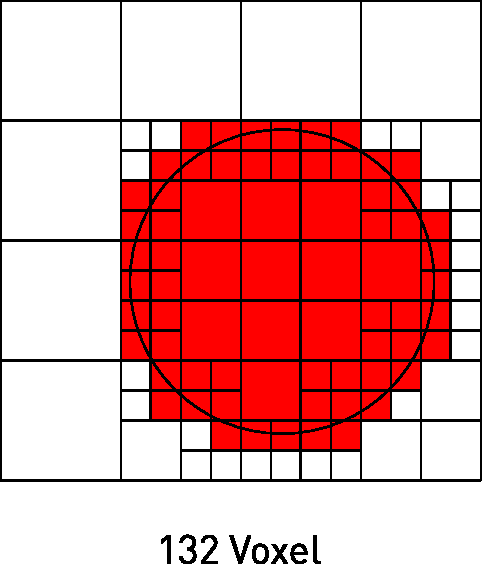
\includegraphics[width=0.32\textwidth]{figures/cut_octree.pdf}
  \caption{Schnitt durch einen Octree \label{cut_octree}}
\end{figure}
Jeder Voxel kann einen oder mehrere Skalare speichern. Oft werden diese Werte nicht direkt im Octree abgelegt um bei die Traversierung der Struktur m�glichst wenig Speicher lesen zu m�ssen. Stattdessen werden die Attributwerte in einem zus�tzlichen Attribut-Buffer abgelegt. In diesem wird f�r jeden Voxel im Octree ein Tupel mit Attributwerten vorgehalten. Die Attribute eines �bergeordneten Voxels ergeben sich im einfachsten Fall aus dem Mittelwerte der Attribute seiner untergeordneten Voxel, vergleichbar mit der Erzeugung von \textit{Mipmaps}. Somit enth�lt jedes Voxel seiner Gr��e entsprechend aufgel�ste Attribut\-werte. Diese approximieren die Auspr�gungen der Attribute innerhalb der r�umlichen Ausdehnung des Voxels. Der Octree bildet also zugleich Geometrie und Textur ab. Der wesentliche Vorteil der Octree-Struktur gegen�ber texturierten Dreiecksnetzen ist, dass sich mit dieser Struktur das LOD-Problem f�r Geometrie und Attribute (Texturen) gleichzeitig l�sen l�sst. Der hierarchische Aufbau und die Granularit�t von Octress erm�glichen eine effiziente Bestimmung der f�r die Darstellung optimale Detailstufe der Daten. Dies kann w�hrend der Bildsynthese durch die Wahl der Traversierungstiefe im Baum pro Bildpunkt geschehen.

\subsection{Verwandte Arbeiten}



%  ////////////////////////////////////////////////////////////////////



\subsection{Sparse Octrees}
F�r einige Anwendungen sind nur bestimmte Auspr�gungen der in den Voxeln gespeicherten Wert von Interesse. Beispielsweise werden beim Iso-Surface-Rendering nur Voxel mit einem bestimmten Dichte\-werte als opake Oberfl�che dargestellt. Werden nur diese Werte ben�tigt, kann die Datenstruktur weiter ausged�nnt werden, indem nur Voxel gespeichert werden die zur Oberfl�che beitragen.
\begin{figure}[position=h]
  \centering
  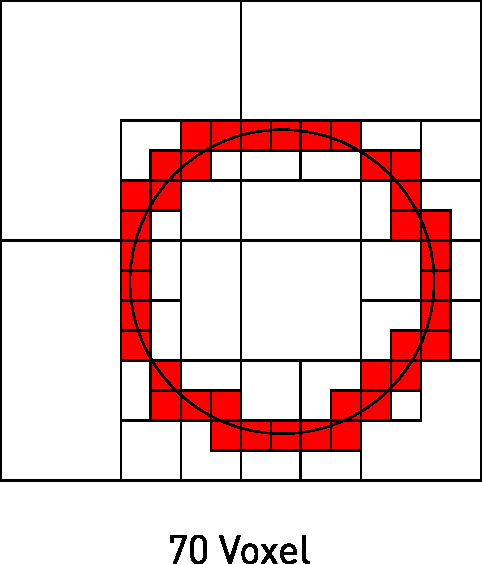
\includegraphics[width=0.32\textwidth]{figures/cut_svo.pdf}
  \caption{Schnitt durch einen Sparse Voxel Octree \label{cut_svo}}
\end{figure}
Eine solche Volumenrepr�sentation eignet sich ebenso zur Darstellung anderer opaker Oberfl�chen wie diskretisierter Dreiecksnetze, Punktwolken oder H�henfeldern und wird als \textit{Sparse Octree} oder \textit{Sparse Voxel Octree} bezeichnet. Innere Knoten k�nnen dabei weniger als acht Kinder haben. Durch die variierende Anzahl von Kindknoten l�sst sich keine implizite Regel zum Berechnen deren Positionen im Speicher herleiten. Vielmehr muss jeder Knoten speichern, welche Kindknoten besetzt sind und wo sich diese im Speicher befinden. Liegen die Kindknoten jedes Voxels jeweils hintereinander im Speicher, muss jedoch nur ein Verweis pro Elternknoten vorgehalten werden. Da in einem Sparse Voxel Octree nur Oberfl�chen gespeichert werden, steigt der Speicherbedarf mit jeder weiteren Tiefenstufe nur durchschnittlich um das vierfache, wie (vgl. ESVORG) zeigen konnte.


\subsection{Verwandte Arbeiten}


%  ////////////////////////////////////////////////////////////////////

\section{Raycasting von Volumendaten}
Bei Raycasting wird f�r jeden Punkt eines Ziel-Buffers ein Strahl erzeugt und mit den Volumendaten geschnitten. 
Volumen\-gitter k�nnen dazu beispielsweise in festen Abst�nden durchschritten werden um Dichtewerte zu ermitteln und �ber eine Transfer\-funktion abzubilden (!!! ABBILDUNG FRONT-TO-BACK-VOLUME-RAYCASTING). Dabei m�ssen auch Bereiche des Volumens verarbeitet werden, die leer sind und nicht zum Bildinhalt beitragen.\\
In der Octree-Darstellung k�nnen gro�e homogen gef�llte Bereiche �bersprungen werden. Dies wird erreicht, indem  der Strahl mit dem Voxel geschnitten wird der diesen Bereich umgibt um so ein Eintritts- sowie ein Austritts\-punkt zu ermitteln. Der hierarchische und regul�ren Aufbau des Octrees erm�glicht es die Anzahl der dazu notwendigen Schnitt\-berechnungen zu minimieren und diese effizient durchzuf�hren. Durch eine Tiefen\-suche im Baum kann in jeder Tiefe das den Strahl zuerst schneidende Voxel ermittelt werden. Da die Voxel ihre Position und Gr��e nur implizit �ber ihrer Lage im Baum speichern, m�ssen diese Werte beim Traversieren f�r jeden Voxel erzeugt werden.\\
\\
Der Strahl kann durch $p_t(t)=p+td$ beschrieben werden. L�st man die Gleichung nach $t$ f�r eine achsen\-parallele Ebene erh�lt man $t_x(x) = (\frac{1}{d_x})x+(\frac{-p_x}{d_x})$.

\begin{figure}[position=h]
  \centering
  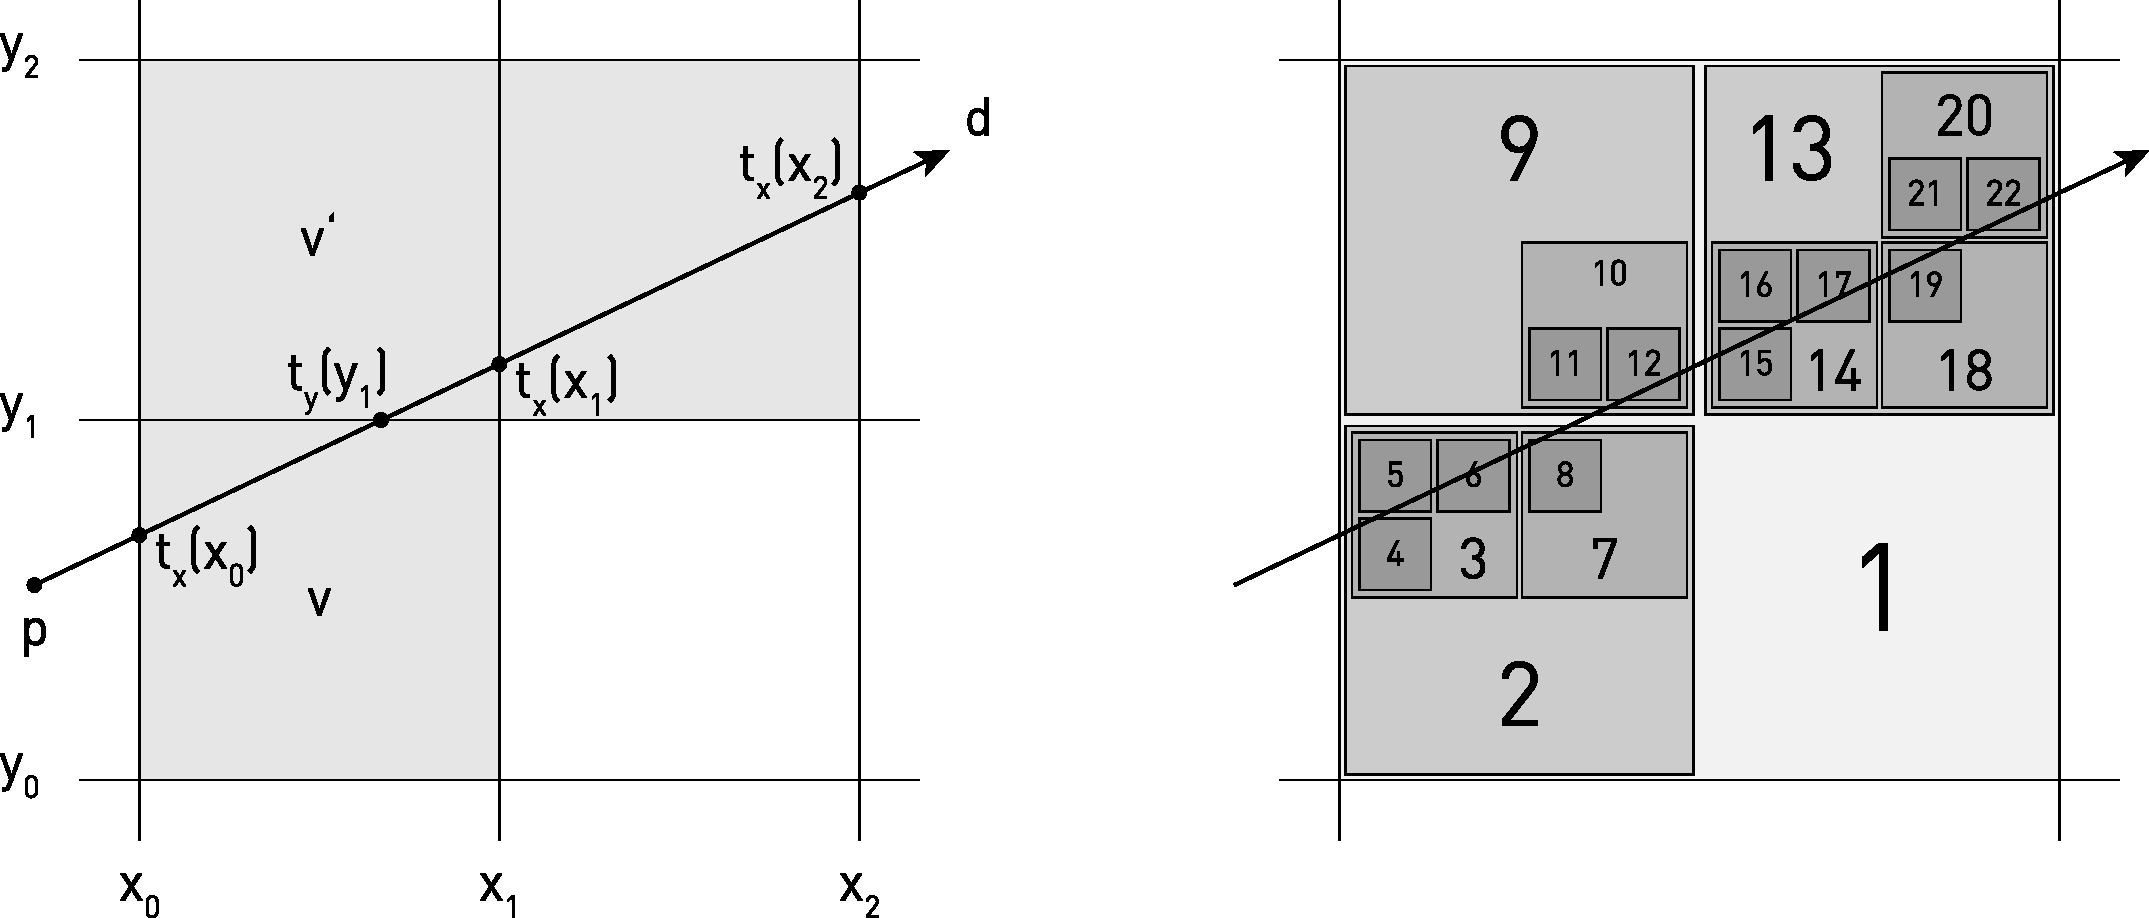
\includegraphics[width=0.75\textwidth]{figures/raycasting.pdf}
  \caption{Bestimmung der Reihenfolge der Kindknoten beim Schnitt \label{raycasting}}
\end{figure}




\subsection{Verwandte Arbeiten}


%  ////////////////////////////////////////////////////////////////////


\section{Out-of-Core Datenmanagement}
Out-of-Core-Strategien erm�glichen einer Anwendung oder einem System die Verwendung von Datenmengen, welche die lokale Speicherkapazit�t �bersteigen. Voraussetzung daf�r ist die Seg\-men\-tier\-bar\-keit der Daten. Au�erdem muss die lokal gespeicherte Untermenge der segmentierten Daten zu jedem Zeitpunkt zur Verarbeitung gen�gen.
\begin{figure}[position=h]
  \centering
  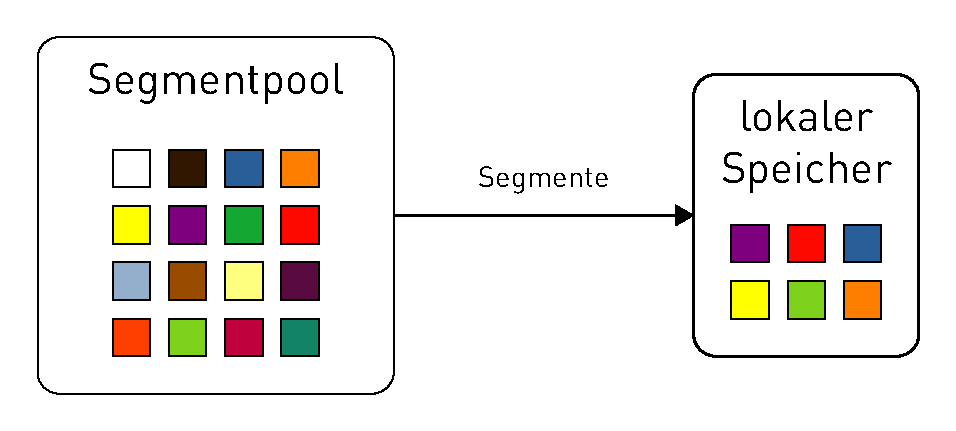
\includegraphics[width=0.75\textwidth]{figures/out_of_core_principal.pdf}
  \caption{Out-Of-Core-Prinzip\label{out_of_core_principal}}
\end{figure}
\\
Die endliche Menge lokalen Speichers der GPU begrenzt die maximale Aufl�sung der SVO-Struktur. Eine Vergr��erung des Speichers l�st das Problem nicht nachhaltig, da wie oben beschrieben eine weitere SVO-Tiefe etwa die vierfache Speicher\-menge ben�tigt.\\
(!!! streaming system notwendig)\\
(beispiele f�r ooc Systeme)\\

\subsection{Verwandte Arbeiten}


%  ////////////////////////////////////////////////////////////////////





\newpage
\chapter{Systemkonzeption}


\section{�berblick}

 - Fehler bei der Darstellung -> Fehlerwert ausnutzen\\
 - Visueller/Progressiver Ansatz (outputsensitiv)\\



\section{Datenstruktur}


\section{Aufbau}
\begin{figure}[position=h]
  \centering
  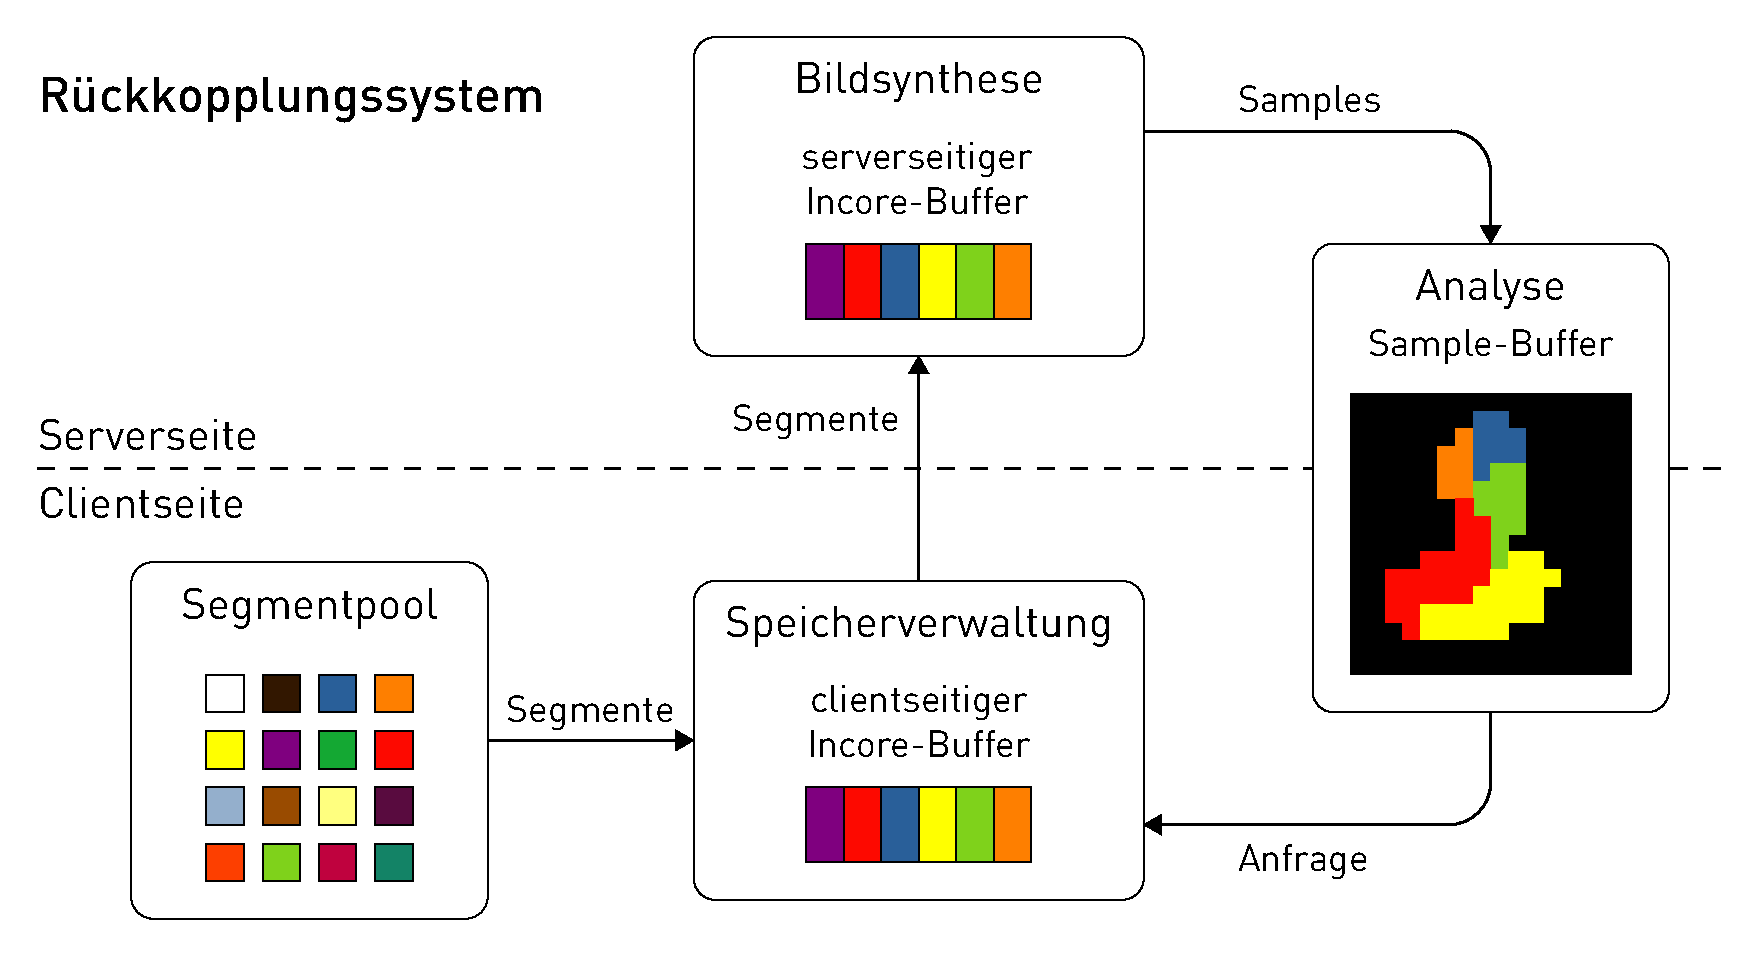
\includegraphics[width=0.85\textwidth]{figures/out-of-core_setup.pdf}
  \caption{Schematischer Aufbau des Out-Of-Core-Systems\label{out-of-core_setup1}}
\end{figure}

\section{Out-of-Core Management}


\section{Real Time Rendering von SVO}

\newpage
\chapter{Implementierungsdetails und Umsetzung}


\section{�berblick}
In den folgenden Abschnitten werden die Abl�ufe zur Erstellung der Octree-Struktur und dem zur dynamischen Anpassung verwendeten Out-of-Core-Ansatzes beschrieben. Dabei soll die Funktionsweise der beteiligten Systemkomponenten beschrieben und deren Implementation an geeigneten Stellen be\-trach\-tet werden.


\section{Aufbau der Sparse Voxel Octree Datenstruktur}





%/////////////////////////////////////////////////////////




%/////////////////////////////////////////////////////////



\subsection{Erzeugung der Treelet Struktur}\label{sec:erzeugung_treelet_struktur}

Die SVO-Struktur wird schon bei der Erstellung segmentiert, das hei�t, in Treelets unterteilt. Sollte der Ar\-beits\-speicher f�r die erzeugten Daten nicht ausreichen, bestht daher die M�glichkeit, bereits erzeugte Treelets auf die Festplatte auszulagern. Im Folgendem soll ein �berblick �ber den Ablauf der Erstellung einer SVO-Struktur aus Treelets gegeben werden. In den folgenden Abschnitten werden die einzelnen Schritte genauer betrachtet.\\\\
Als Eingabe werden zun�chst die geforderte minimale Tiefe des resultierenden Octrees, die Speichergr��e der Treelets und der Pfad zu den Eingabedaten ben�tigt. Der Build-Manager erstellt ein initiales, leeres Treelet (\textit{Wurzel-Treelet}) und �bergibt dieses an den Treelet-Builder. Dieser f�llt das Treelet anhand der Eingabedaten. Anschlie�end werden alle entstandenen Blatt-Knoten, die noch nicht die geforderte, minimale Tiefe in der Octree-Struktur aufweisen, notiert. Zu jedem dieser Blattknoten wird eine Liste der in ihm liegenden Primitive der Eingabedaten gespeichert. Zus�tzlich wird auch die Tiefe des Knotens im Baum und seine Transformation relativ zum Wurzelknoten notiert. Um die Verkn�pfung der Treelets untereinander realisieren zu k�nnen wird au�erdem der Treelet-Index, der Index des Blattknotens und dessen Elternknotens gespeichert (vgl. Abschnitt \ref{sec:segmentierung} \nameref{sec:segmentierung}, Seite \pageref{sec:segmentierung}). Der Build-Manager speichert diese Informationen in einer Queue und erzeugt f�r jeden Eintrag ein neues Treelet (\textit{Top-Down}). Diese neuen Treelets werden durch die gespeicherten Treelet- und Blattknotenindices des Wurzel-Treelets initialisiert und sind so logisch mit diesem verbunden. Jedes dieser Treelets wird wiederum dem Treelet-Builder �bergeben, der es anhand seiner Primitivliste und der gespeicherten Transformation mit Voxeln f�llt. Der Build-Manager erzeugt sukzessiv weitere Treelets aus Blattknoten bereits erstellter Treelets bis die geforderte minimale Tiefe des Octrees f�r alle Blattknoten erreicht ist.
\begin{figure}[position=h]
  \centering
  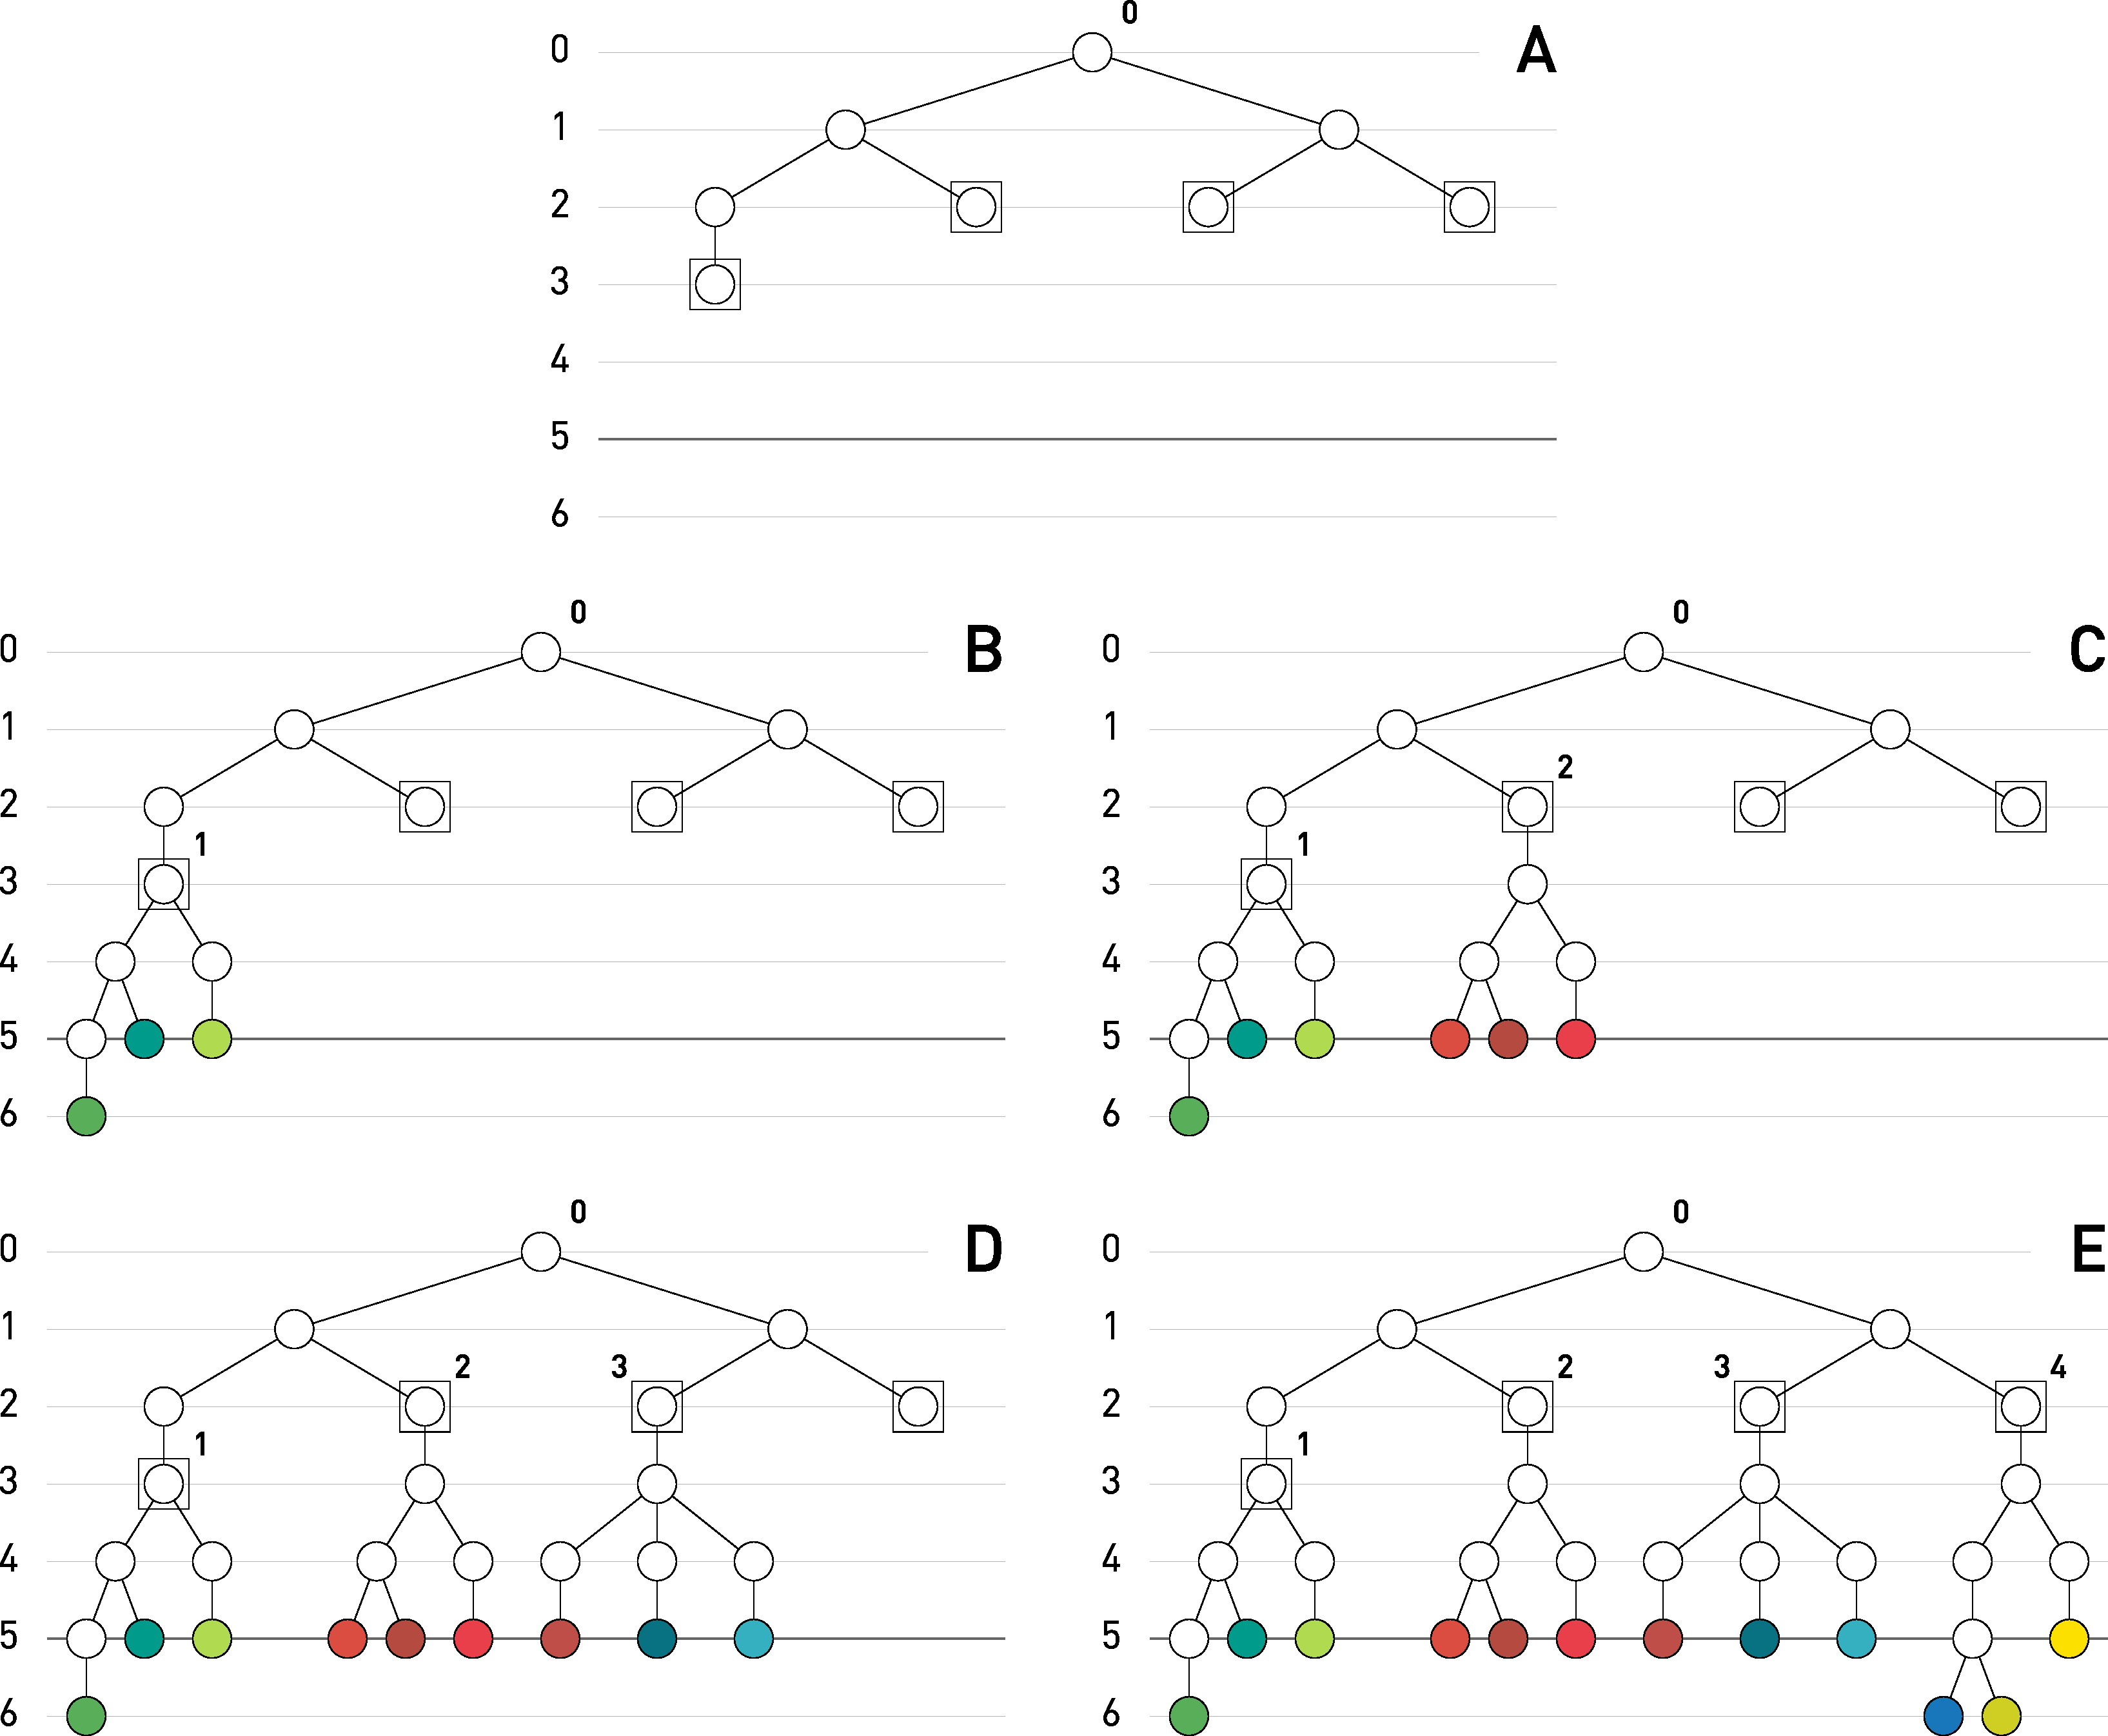
\includegraphics[width=0.83\textwidth]{figures/treelet_building.pdf}
  \caption{Schrittweiser Aufbau der SVO-Struktur aus Treelets \label{fig:treelet_building}}
\end{figure}
\newpage
F�r Blattknoten mit ausreichender Tiefe erzeugt ein Attributgenerator die gew�nschten Attribute und speichert diese in einem zus�tzlichen Buffer. Die Primitiv\-liste sowie alle weiteren Informationen, die zur Erstellung weiterer Treelets ben�tigt w�rden, k�nnen an dieser Stelle verworfen werden. Abbildung \ref{fig:treelet_building} zeigt den schrittweisen Aufbau eines Octrees aus Treelets.\\
Ist die Erstellung der Treelets abgeschlossen, werden die Attribute der inneren Knoten durch Mitteln der Attribute ihrer Untergeordneten Knoten erstellt. Dies geschieht f�r alle Treelets in umgekehrter Reihenfolge ihrer Erstellung (\textit{Bottom-Up}). So wird sichergestellt, dass der Wurzelknoten eines untergeordneten Treelets bereits Attributinformation enth�lt, wenn sein �bergeordnetes Treelet diese zur Generierung der Attribute in seinen Blattknoten ben�tigt. Mit der Erstellung der Attribute in dem Wurzelknoten des Wurzel-Treelets ist die Erstellung des Octrees abgeschlossen. 




%/////////////////////////////////////////////////////////



\subsection{Treelet Aufbau}
Der Treelet-Builder erstellt die Knoten in der Breite (\textit{Breadth-First}) und arbeitet dazu intern auf einem FIFO-Container (\textit{Queue}). Der Aufbau eines Elementes dieser Queue ist im Listing \ref{lst:queueelement} zu sehen. Jedes Element der Queue entspricht einem Knoten in der SVO-Struktur und enth�lt alle n�tigen Informationen, um diesen Knoten seinem �bergeordneten Knoten mitzuteilen sowie die Erzeugung weiterer Unterknoten zu erm�glichen.

%\begin{figure}[position=h width=0.75\textwidth]
%  \centering
\begin{lstlisting}[caption={Queue-Element},label={lst:queueelement}]
struct QueueElement
{
  // Knoten-Index des Knotens innerhalb des Treelets
  unsigned              _localLeafIndex;         
  // Kind-Index des Knotens innerhalb seines Eltern-Knotens
  char                  _idx;                    
  // Knoten-Index des Eltern-Knotens
  unsigned              _parentLocalNodeIndex;   
  // Tiefe des Knotens in der SVO-Struktur
  unsigned              _depth;                  
  // Transformation des Knotens relativ zum Wurzelknoten
  gloost::Matrix        _aabbTransform;          
  // In diesem Knoten enthaltene Primitive der Ausgangsdaten
  std::vector<unsigned> _primitiveIds;           
};
\end{lstlisting}
%\end{figure}
Initial wird ein Queue-Element stellvertretend f�r den Wurzelknoten des aktuellen Treelets erstellt. Dieses enh�lt die relative Transformation des Knotens in der SVO-Struktur sowie alle Primitive, die in diesem Knoten liegen. F�r jeden potentiellen Kind-Knoten wird ein Queue-Element mit entsprechenden Parametern erzeugt und dessen \textit{Bounding Box} mit  Primitiven des aktuellen Queue-Elementes zum Schnitt gebracht. Dabei wird f�r jeden Kindknoten die Untermenge an Primitiven notiert, die geschnitten wurden. Falls ein Kindknoten keine Primitive enth�lt, wird es verworfen. Kindknoten, die Primitive enthalten, erhalten aufeinanderfolgende Speicherpositionen innerhalb des Treelets.\\
Die Position des ersten Kindknotens wird im \textit{First-Child-Index} des Knotens des aktuellen Queue-Elements gespeichert. Nun werden die Queue-Elemente der Kindknoten zur weiteren Verfeinerung in die Queue eingereiht. Vor dem Abarbeiten eines Queue-Elementes wird �berpr�ft, ob im Treelet noch gen�gend freie Pl�tze f�r eine weitere Unterteilung vorhanden sind. Sind weniger als acht Pl�tze �brig, muss nach der n�chsten Unterteilung erst �berpr�ft werden, ob die entstanden Kindknoten noch in das Treelet passen, bevor die Unterteilung gespeichert werden kann. Ist dies nicht der Fall, wird versucht ein Queue-Element zu finden, dessen Bearbeitung weniger neue Knoten erzeugt. Kann kein solches Queue-Element gefunden werden, ist die Erstellung des Treelets abgeschlossen.\\
Die in der Queue verbliebenen Elemente werden nach ihrer Baumtiefe in finale und weiter zu unterteilende Elemente getrennt und in zwei Containern im Treelet gespeichert. Nachdem die finalen Knoten in den Leaf-Masks der Eltern-Knoten als solche markiert wurden, wird das Treelet an den Build-Manager zur�ckgegeben.\\\\
Der Build-Manager erzeugt f�r jedes nicht finale Queue-Element ein weiteres Treelet. Der Indices der neu erstellten Treelets werden im \textit{First-Child-Index} der zugeh�rigen Blattknoten des �bergeordneten Treelets gespeichert. Jedes dieser Treelets wird mit einer Primitivliste, seiner Transformation und dem Eltern-Treelet-Index parametrisiert in der Queue des Build-Managers einge\-reiht um sie in entsprechender Reihenfolge an den Treelet-Builder weitergeben zu k�nnen. Der oben beschriebene Ablauf wiederholt sich daraufhin f�r jedes Treelet in der Queue. Liefert der Treelet-Builder nur noch Treelets mit finalen Blattknoten, leert sich die Queue und das Erstellen der SVO-Struktur ist abgeschlossen. 


%/////////////////////////////////////////////////////////


\subsection{Attribut-Generierung}
Zu jedem Treelet werden parallel ein oder mehrere Buffer mit verschachtelten (\textit{interleaved}) Attributwerten erstellt. Die Verschachtelung sorgt f�r einen speicherkoh�renten Zugriff auf alle Attributwerte eines Voxels. Anzahl und Layout der Attribut-Buffer sind abh�ngig vom gew�hlten Attribut-Generator.\\
F�r jeden finalen Blattknoten wird mit Hilfe der gespeicherten Primitive und Transformation eine Menge von Attributen erzeugt. Dieser Vorgang soll im Folgenden am Beispiel von Dreiecks\-primitiven erl�utert werden. F�r jedes Dreieck innerhalb eines Blatt-Knotens wird ein Strahl erzeugt, der durch die Voxel\-mitte und senkrecht zum Dreieck verl�uft (vgl. Abbildung \ref{voxel_primitiv_schnitt}a). Es werden die Schnittpunkte des Strahls mit dem Dreieck ermittelt, um damit UV-Koordinaten berechnen zu k�nnen.
\begin{figure}[position=h]
  \centering
  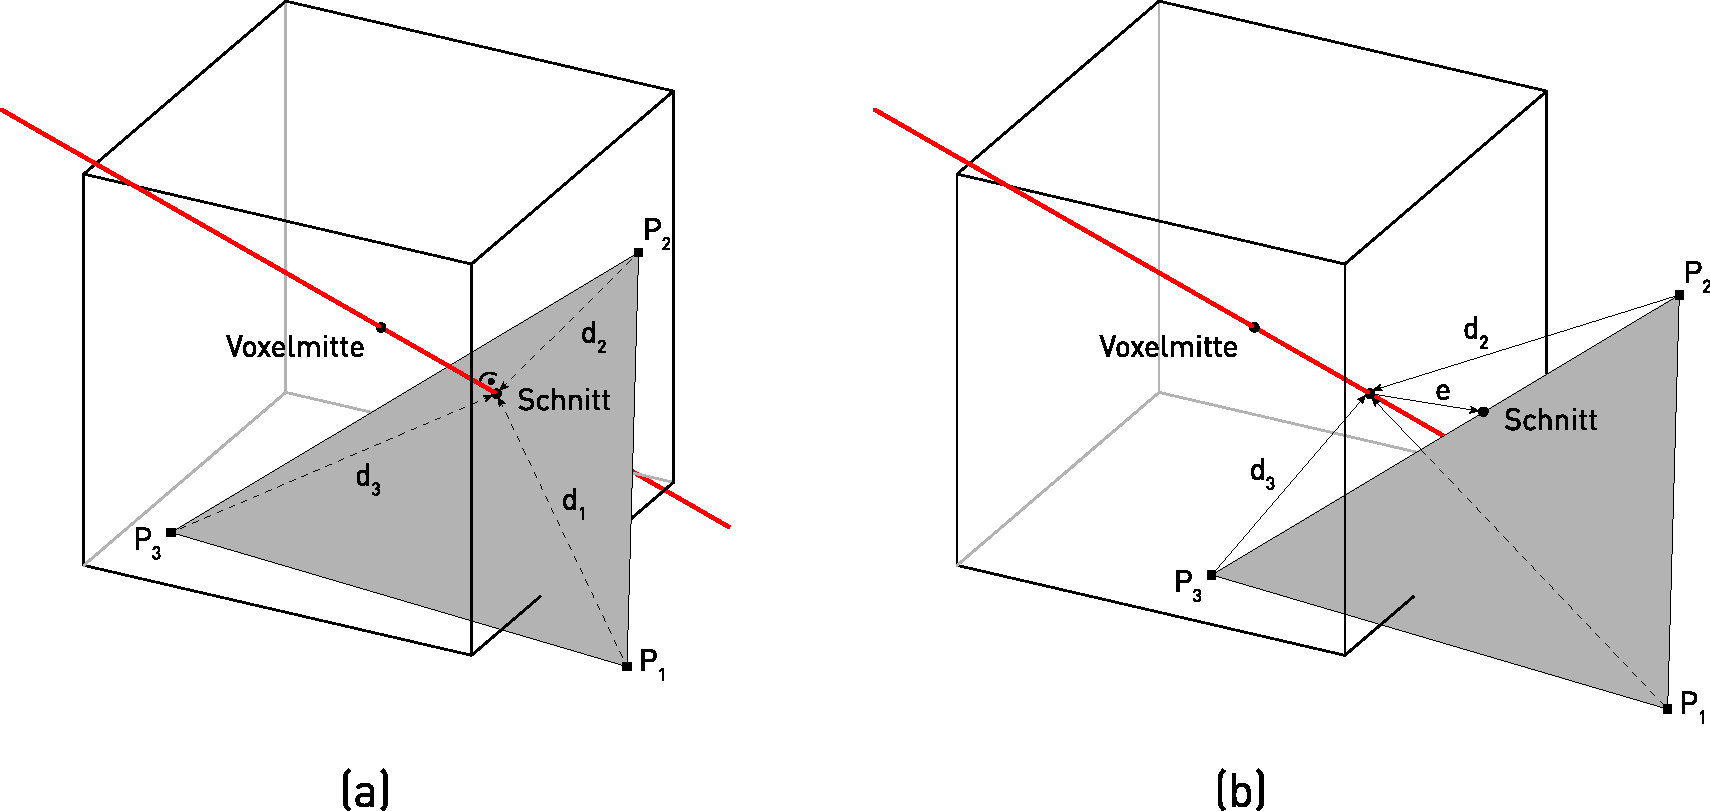
\includegraphics[width=0.85\textwidth]{figures/voxel_primitiv_schnitt.pdf}
  \caption{Ermittlung von UV-Koordinaten\label{voxel_primitiv_schnitt}}
\end{figure}
Durch die senkrechte Ausrichtung des Strahls zur Dreicks\-fl�che wird die Wahrscheinlichkeit eines Schnittes erh�ht. Trotzdem ist es m�glich, dass der Strahl das Dreieck verfehlt, da das Voxel das Dreieck bei\-spiels\-weise nur mit einer Ecke schneidet, die nicht zur Voxel-Mitte ausgerichtet ist (vgl. Abbildung \ref{voxel_primitiv_schnitt}b). Um trotzdem den Beitrag des Dreiecks zu den Voxel-Attributen ber�cksichtigen zu k�nnen,  wird in diesem Fall der Punkt auf dem Dreieck als Schnittpunkt angenommen, der den kleinsten Abstand zum Schnittpunkt mit der Dreiecksebene besitzt. Dieser Vorgang erzeugt ein Rauschen in den Daten, das aber angesichts der geringen Gr��e der Blatt-Knoten und des daraus resultierenden geringen Fehlers keinen nennenswerten Einfluss auf die subjektive Bildqualit�t hat. Mit Hilfe der ermittelten UV-Koordinaten k�nnen nun Attribute wie Farbe oder Richtung aus den Eckpunkten der Dreiecke interpoliert oder aus Texturen gelesen werden. Aus den Werten aller am Voxel beteiligten Dreiecke wird ein Mittelwert gebildet. Farb- und Richtungs\-werte werden auf 8 Bit pro Komponente quantisiert bevor sie in den Attributbuffer gespeichert werden.\\
\newpage
Wie in Abschnitt \ref{sec:erzeugung_treelet_struktur} beschrieben, werden die Attribute der inneren Knoten erst erzeugt, nachdem die Erstellung aller Treelets ab\-ge\-schlos\-sen ist. Durch die Verwendung eines FIFO-Containers im Build-Manager sind die Treelets so nummeriert, dass jedes Treelet einen niedrigeren Index besitzt als seine untergeordneten Treelets. Das Treelet mit dem h�chsten Index besitzt schon in allen seinen Blatt-Knoten Attribute und ist somit von keinem anderen Treelet f�r die Generierung seiner Attribute abh�ngig. Das Treelet mit dem Index $0$ ist dagegen f�r seine Attributgenerierung von allen anderen Treelets abh�ngig. F�r die Generierung der Attribute werden die Treelets daher in umgekehrter Reihenfolge ihrer Indizierung verarbeitet. Abbildung \ref{attribute_generation} veranschaulicht die Reihenfolge anhand eines Beispiels (vgl. Abbildung \ref{fig:treelet_building}).
\begin{figure}[position=v]
  \centering
  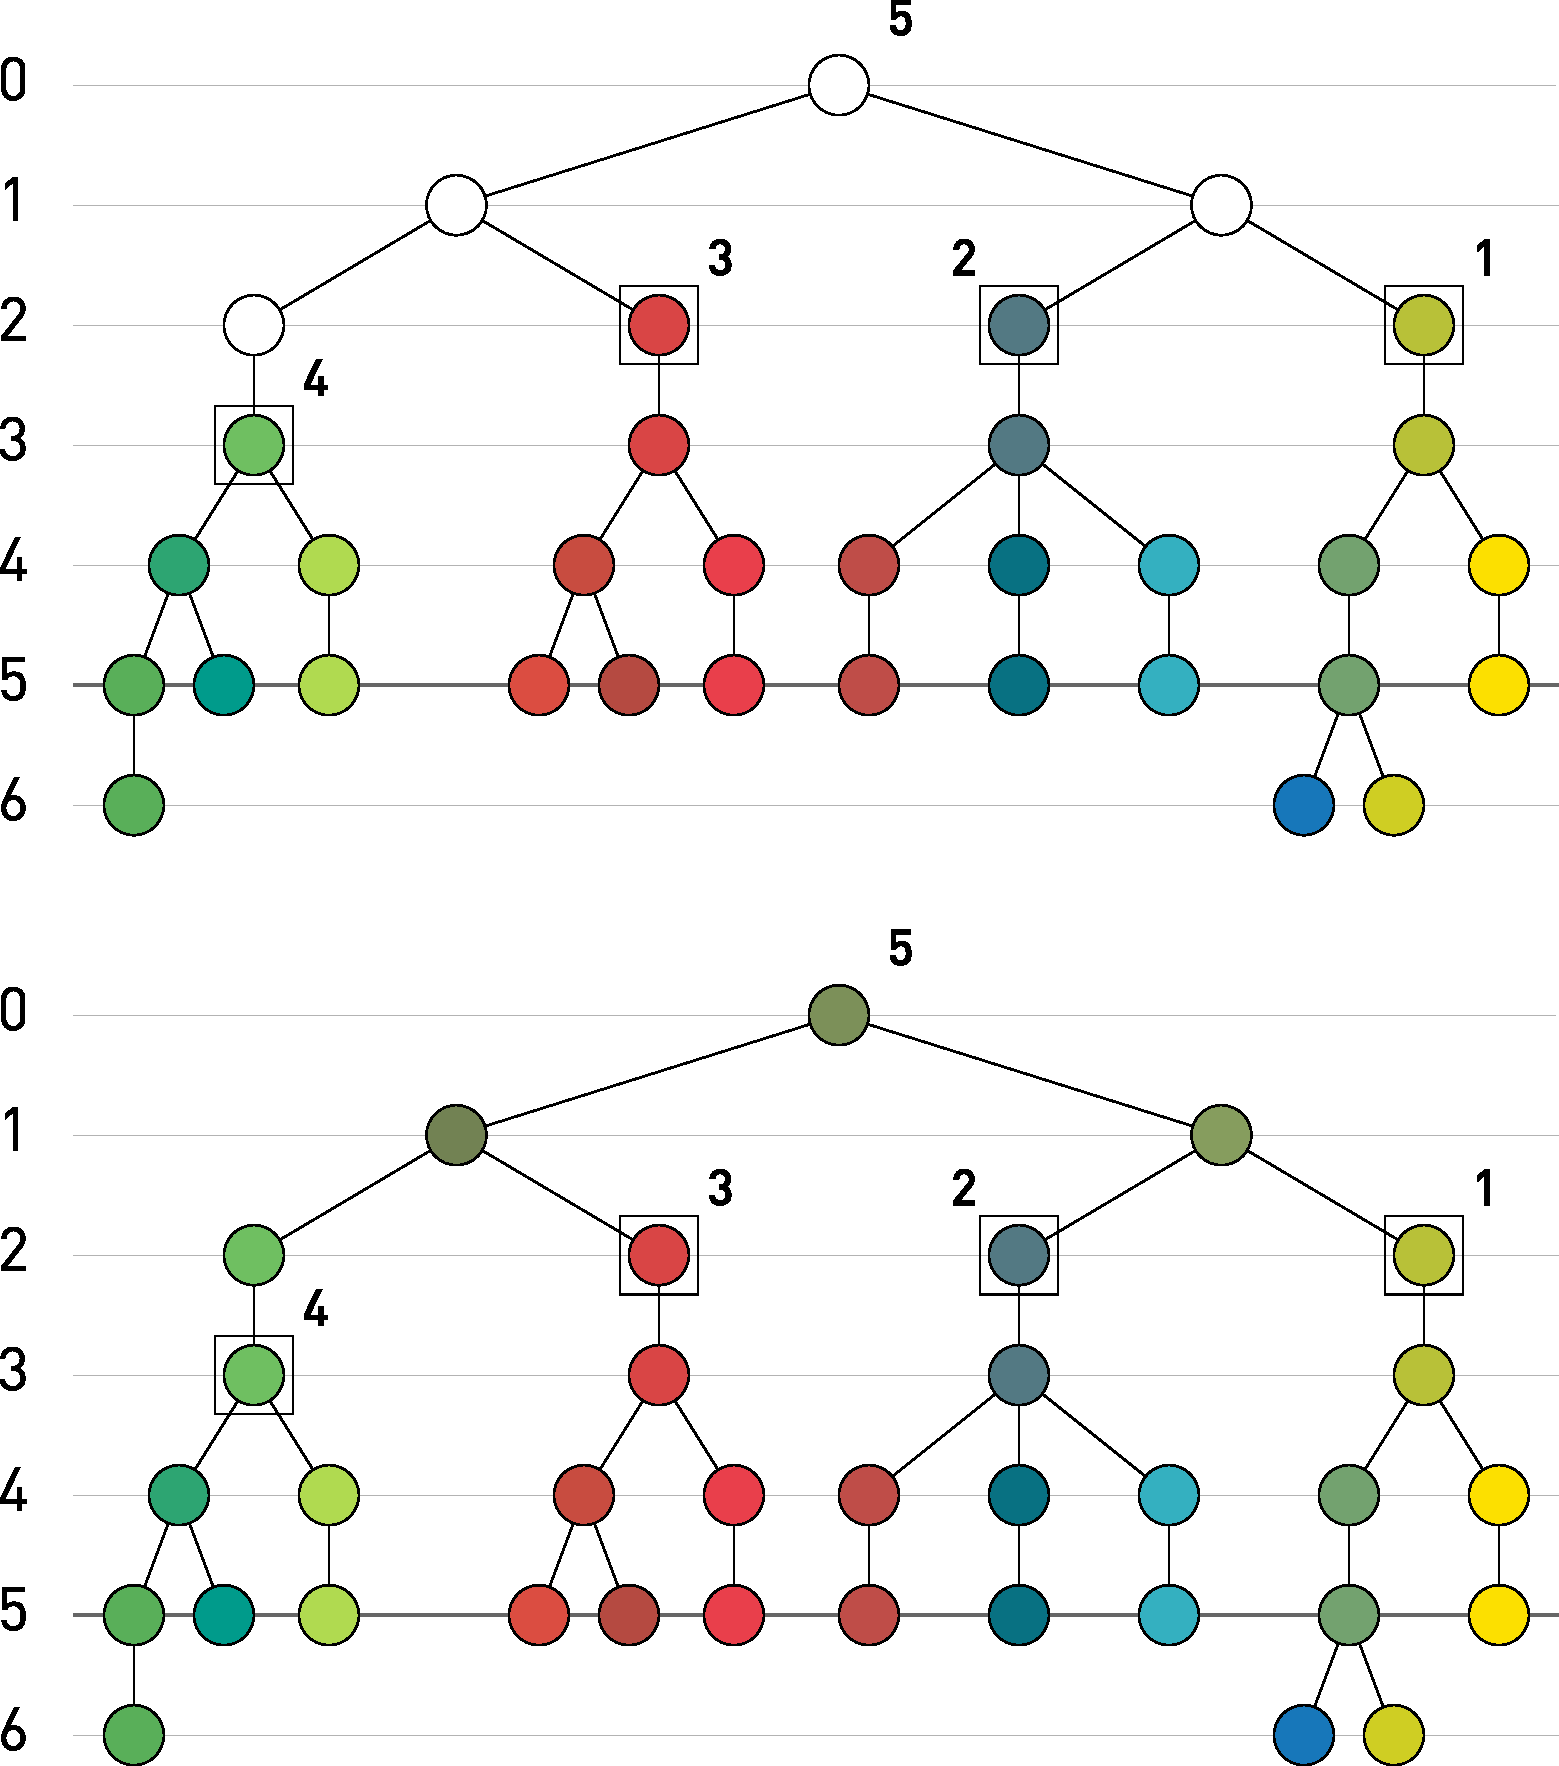
\includegraphics[width=0.70\textwidth]{figures/attribute_generation.pdf}
  \caption{Reihenfolge der Erzeugung der Attributen innerer Knoten\label{attribute_generation}}
\end{figure}\\
Beginnend beim Treelet mit dem gr��ten Index wird jedes Treelet vom Wurzelknoten an der Tiefe nach rekursiv durchlaufen bis die Blattknoten erreicht werden. Beim Aufsteigen aus der Rekursion wird aus den Attributen der  vorhandenen Kindknoten ein Mittelwert gebildet und im Attribut-Buffer abgelegt. Dazu werden die mit 8 Bit aufgel�sten Attribut\-komponenten der Kindknoten zun�chst wieder in 32 Bit Flie�\-komma\-werte konvertiert, um die Quantisierungsfehler bei der Ermittlung des Mittelwerts nicht unn�ig zu verst�rken. Nachdem auch f�r den Wurzelknoten ein Attribut vorhanden ist, wird dieses in den Attribut-Buffer des �bergeordneten Treelets f�r den entsprechenden Blattknoten abgelegt. Durch die Reihenfolge der Indizierung ist f�r jedes Treelet sichergestellt, dass f�r alle Blatt\-knoten Attributinformationen vorhanden sind wenn sie zur Generierung der Attribute der inneren Knoten ben�tigt werden.




\newpage

\section{Echtzeitf�higes SVO-Ray Casting}


\subsection{Prinzipieller Aufbau}

Der in dieser Arbeit verwendete Out-Of-Core-Ansatz besteht grunds�tzlich aus vier Teilen (Abbildung \ref{out-of-core_setup}): Einem gro�en, clientseitigen \textbf{Segmentpool} der die gesamte SVO-Struktur vorh�lt, einem vergleichsweise kleinen Buffer der eine Untermenge der SVO-Struktur halten kann und auf Server- und Clientseite existiert (\textbf{\textit{Incore-Buffer}}), einer \textbf{Speicherverwaltung} die den server-seitigen Buffer pflegt und einem \textbf{Analysesystem} das entscheidet welche Segmente ben�tigt werden.
\begin{figure}[position=h]
  \centering
  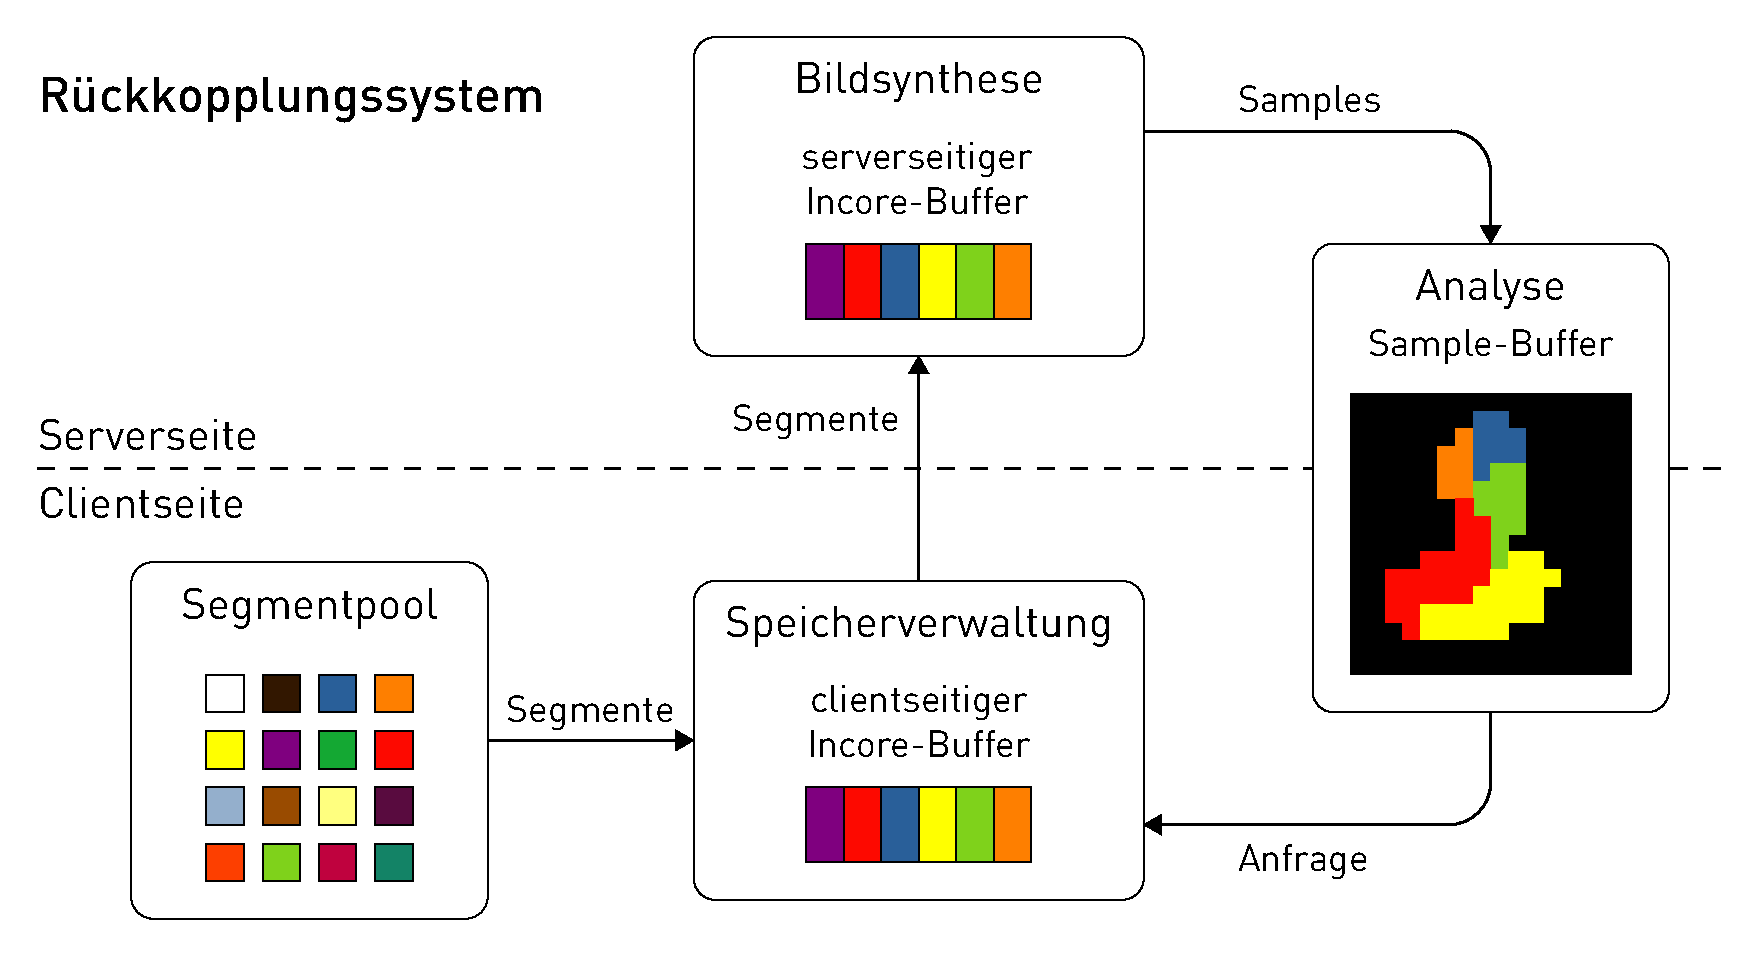
\includegraphics[width=0.85\textwidth]{figures/out-of-core_setup.pdf}
  \caption{Schematischer Aufbau des Out-Of-Core-Systems\label{out-of-core_setup}}
\end{figure}
Der Incore-Buffer, der auf Client- und Serverseite vorhanden ist, wird wie der SVO in Segmente gleicher Gr��e (\textbf{\textit{Slots}}) aufgeteilt von denen jeder ein Treelet aufnehmen kann. Die Wahl einer einheitliche Treelet- und Gr��e verhindert somit Fragmentierung des Incore-Buffer und entsprechenden Aufwand zu Defragmentierung. Die Analyse arbeitet serverseitig auf den im Incore-Buffer vorhandenen Treelets. (!!! WEITER)



% ////////////////////////////////////////////



\subsection{�berblick der Verarbeitungsschritte}
Im Folgendem soll der Ablauf der dynamischen Ver�nderung der SVO-Struktur im Incore-Buffer, abh�ngig von der Kameraposition erl�utert werden. In den folgenden Kapiteln wird auf die einzelnen Schritte genauer eingegangen.\\
Der Incore-Buffer wird zun�chst mit dem Wurzel-Treelet im ersten Slot initialisiert. Die adaptive Anpassung der Baumstruktur wird in vier Schritten realisiert: Zun�chst wird der Octree aus der Sicht der Kamera in den Feedback-Buffer gerendert (\textbf{\textit{Analyse-Pass}}). Nach diesem Schritt enth�lt dieses Buffer f�r jeden Strahl u.A. die Position des getroffenen Knoten im Incore-Buffer und einen Fehlerwert. War der getroffene Knoten ein Blatt, zu dessen Verfeinerung ein Treelet vorhanden ist, wird zus�tzlich noch dessen Index gespeichert.\\
Nach der �bertragung des Feedback-Buffers in den Hauptspeicher werden dessen Eintr�ge in zwei Container verarbeitet (\textbf{\textit{Vorsortierung}}). Der eine enth�lt die Treelet-Indices aller Knoten die getroffen wurden und zus�tzlich die Treelet-Indices ihrer �bergeordneten Treelets bis zum Wurzel-Treelet. Der andere Container enh�lt Anfragen nach Verfeinerung in Form der Treelet-Indices der anzuh�ngen Treelets. Die Fehlerinformation bleibt dabei in beiden Containern erhalten.\\
Jetzt werden beide Container dem Speichermanagement �bergeben(\textit{\textbf{clientseitige Aktualisierung}}). Dort werden zun�chst die Sichtbarkeitsinformation aller im letzten Zyklus gesehenden Treelets aktuallisiert. Danach werden die neu anzuh�ngenden Treelets in den clientseitigen Incore-Buffer eingepflegt. Dabei werden nicht sichtbare Treelets entfernt falls im Incore-Buffer keine freien \textit{Slots} mehr zur Verf�gung stehen. Ge�nderte Slots werden markiert. Abschlie�end werden die ver�nderten Bereiche des Incore-Buffers an den Server �bertragen und stehen nun dem Renderer f�r den n�chsten Zyklus zur Verf�gung (\textbf{\textit{serverseitige Aktualisierung}}).\\
Die folgenden Abschnitte werden diese Schritte genauer betrachten.



% ////////////////////////////////////////////



\subsection{Analyse Pass}
Um die Last, die durch diesen zus�tzlichen Render-Pass entsteht, m�glichst gering zu halten ist die Gr��e des zur Analyse verwendeten Zielbuffer wesentlich kleiner als die des f�r die Bildgenerierung verwendete Frame-Buffers. Um Artefakt\-bildung zu vermindern werden die Strahlen bei jedem Analyseschritt durch Zufalls\-werte parallel zur Sicht-Ebene verschoben. Die Verschiebung ist dabei so gew�hlt das �ber die Zeit im Bereich von $nxn$ Frame-Buffer Texeln abgetasted wird wobei $n$ das Verh�ltnis der Gr��en von Frame-Buffer und Analyse-Buffer ist.
Damit ist es m�glich den Analyse-Buffer auf bis $1/8$ der G��e des Frame-Buffers zu verkleinert ohne das es durch Aliasing zu Artefaktbildung kommt oder zu wenig Information zur Verf�gung steht um die nachfolgende dynamische Anpassung des Octrees zu treiben.\\

Das F�llen des Feedback-Buffers erfolgt analog zum bilderzeugenden Raycasting in OpenCl auf dem im Incore-Buffer vorhanden Octree. Nach der Traversierung des Octrees liegt f�r jeden Strahl eines der folgenden drei Ergebnisse vor:  
\begin{enumerate}
  \item der Strahl trifft nicht  
  \item der Strahl trifft einen inneren Knoten
  \item der Strahl trifft ein Blatt
\end{enumerate}
Im ersten Fall wird nichts zur�ckgegeben, im Zweiten nur die Position des Voxels im Incore-Buffer und die L�nge des Strahles. Im dritten Fall wird zus�tzlich der Verweis auf ein evt. vorhandenes Sub-Treelet und die Differenz zwischen vorgefundener Voxelgr��e und der f�r die L�nge des Strahles idealen Voxelgr��e als Fehlerwert gespeichert.

\begin{lstlisting}[caption=Struktur eines Feedback-Elementes]{structFeedBackDataElement}
  struct FeedBackDataElement
  {
    // Knoten-Index im Incore-Buffer in dem der Strahl terminierte
    int   _nodeId;
    // Unterschied zwischen geforderter und erreichter Voxelgr��e
    float _error;
    // Treelet-Index, falls der Strahl in einem Blatt terminierte
    int   _subTreeletGid;
    // Entfernung von Kamera und Knoten (nicht notwendig f�r den beschriebenen Ablauf)
    float _tmin;
  };
\end{lstlisting}


\subsection{Vorsortierung}

Nach dem Transfer des Analyse-Buffers vom Server in den Hauptspeicher, werden dessen Elemente ausgewertet. Dabei werden zwei Container mit unterschiedlichen Sichtinformationen gef�hlt. Im ersten Container werden Indices von Treelets notiert, die bereits im Incore-Buffer vorhanden sind, im Zweiten nur Anfragen nach neuen Treelets. Beide Container sind nach dem Fehlerwert der Eintr�ge absteigend sortiert wobei jeder Treelet-Index �ber beide Container hinweg unique ist.\\
Im oben beschriebenen Fall 1 (der Strahl trifft nicht) liegen keine Sichtbarkeitsinformation vor weshalb solche Eintr�ge �bersprungen werden. Im Fall 2 (der Strahl trifft einen inneren Knoten) wird �ber die erhaltene Position des Knoten im Incore-Buffer und �ber die Gr��e eines Treelets auf den \textit{Slot} des zugeh�rigen Treelets und damit auch auf den entsprechenden Treelet selbst geschlossen. Durch die in den Treelets gespeicherten Eltern-Information werden zus�tzlich alle �bergeordneten Treelets als sichtbar notiert. Tritt bei der Notation ein Treelet mehrfach auf, wird jeweils der gr��te Fehler notiert.\\
Im Fall 3 (der Strahl trifft ein Blatt) wird f�r den Blattknotenindex wie im Fall 2 vorgegangen. Zus�tzlich wird der Treelet-Index des anzuh�ngenden Treelets im entsprechenden Container gespeichert. Tritt ein Treelet-Index mehrfach auf wird auch hier nur ein Eintrag mit dem gr��ten Fehler gespeichert.\\
Nachdem alle Elemente des Feedback-Buffers verarbeitet wurden werden beide Container dem Speichermanager �bergeben.



% ////////////////////////////////////////////



\subsection{Clientseitige Aktualisierung}
Die Pflege der Sichtbarkeitsinformationen der bereits im Incore-Buffer befindlichen Treelets ist trivial: Zun�chst wird die Sichtbarkeit jedes \textit{Slots}, d.h. die Sichtbarkeit jedes im \textit{Incore-Buffer} befindlichen Treelets dekrementiert. Dann wird die Sichtbarkeit derjenigen Treelets aktualisiert, die beim letzten Analyse-Pass gesehen wurden. Dabei wird die Sichtbarkeit auf einen vorher festgelegten Maximalwert gesetzt der dem Gr��enverh�ltnis von Render-Buffer und Analyse-Buffer entspricht. %Da die Anzahl der berechneten Samples im Analyse-Buffer bei einem Gr��enverh�ltnis von $1/8$ nur einem $1/64$ der berechneten Pixel im Framebuffer entspricht w�hre anzunehemen das die miximale Sichtbarkeitswert h�her sein m�sste. 

\subsection{Einf�gen eines Treelets}
F�r das Einf�gen eines Treelts aus dem in der Vorsortierung erstellten Containers wird zun�chst ein freier Slot innerhalb des Incore-Buffers ben�tigt. Ist dieser vorhanden kann das Treelet an die ensprechende Stelle im Incore-Buffer kopiert werden. Der Slot-Index wird im Treelet-Objekt gespeichert und zur Aktuallisierung des serverseitigen Incore-buffers vorgemerkt. Die folgende Ver�nderung der Baumstruktur kann in Listing \ref{lst:insert_treelet} nachvollzogen werden. Aus dem Treelet werden folgende Informationen gelesen:
\begin{enumerate}
  \item der Treelet-Index des Eltern-Treelets
  \item der Knoten-Index des Blattes, an dem das Treelet angeh�ngt werden soll
  \item der Eltern-Knoten-Index des Blattes
  \item die Position des Blattes in seinem Eltern-Knoten
\end{enumerate}
Damit wird nun die Position des entsprechenden Blatt\-knotens des Eltern-Treelets im Incore-Buffer ermittelt und durch den Wurzel\-knoten des anzuh�ngenden Treelets ersetzt. Dadurch muss dessen relative Index zu seinem ersten Kindknoten angepasst werden. Der erste Kindknoten des neuen inneren Knotens findet sich immer an zweiter Position innerhalb des angeh�ngten Treelets im Incore-Buffer. Der Blattknoten wird damit zu einem inneren Knoten, was wiederum in seinem Elternknoten an der ensprechenden Stelle in der \textit{Childmask} markiert wird. In einem weiteren Container wird vermerkt, dass das Parent-Treelet nun ein neues Kind-Treelet im Incore-Buffer besitzt. Abschlie�end wird der Slot-Index des Parent-Treelets zur sp�teren serverseitigen Aktualisierung vorgemerkt. 
\lstinputlisting
    [caption={Einf�gen eines Treelets}
       \label{lst:insert_treelet},
       captionpos=t,language=C++]
 {listings/insert_treelet.cpp}
 


% ////////////////////////////////////////////



\subsection{Entfernen eines Treelets}
Ist f�r das Einf�gen eines Treelets kein Slot mehr verf�gbar muss zun�chst ein Slot dessen Treelet nicht sichbar war wieder frei gegeben werden. Dazu wird der Baum der Treelets in einem Thread durchsucht und eine Menge von Kandidaten f�r das Entfernen vorgehalten. Da diese Suche nebenl�ufig geschiet ist nicht sichergestellt, dass dieser Kaditat zum Zeitpunkt des Entfernens noch valide ist. Deshalb muss vor dem eigentlichen Entfernen der Sichtbarkeitswert des Slots zun�chst erneut �berpr�ft werden. Ausserdem ist es m�glich, dass zwar das entsprechende Treelet selbst nicht sichtbar war, jedoch im Falle des Entfernens der entsprechende Blatt-Knoten des Eltern-Treelts. Bild (!!!BILD EINF�GEN) illustriert diesen Fall der ausnahmslos an den R�ndern der Geometry auftritt. Im Bild befindet sich ein geladenes Treelet hinter einer konvexen W�lbung der Geometry und kann so nicht vom Analyse-Pass gesehen werden. Wird dieses Treelt jedoch entfernt, ragt der entstehende Blatt-Knoten des Eltern-Treelets �ber die W�lbung hinaus. Im n�chsten Zyklus w�rde dieses Blatt wieder verfeinert werden wodurch es zu flackernden Artefakten an den Geometrie\-kanten kommt. Um diese Artefaktbildung zu verhindern werden Umgebungsinformationen, sprich die Sichtbarkeit des Eltern-Treelts mit�berpr�ft. Nur wenn auch das Eltern-Treelet nicht sichtbar ist, kann das Treelet sicher entfernt werden.\\
Alle Slots von im Incore-Buffer gespeicherten Treelts die sich unterhalb des zu entfernenden Treelts befinden k�nnen sofort freigegeben werden. Dazu wird die Kind-im-Incore-Buffer-Information des Kan\-di\-daten-Treelets und rekursiv die aller untergeordneten Treelets traversiert. So werden im g�nstigen Fall gleich mehrere Slots freigegeben.\\
Die Manipulation des Incore-Buffers zum Entfernen des Kan\-di\-daten-Treelets l�uft weitestgehens analog zum Einf�gen ab. Die folgenden Schritte k�nnen im Listing \ref{lst:remove_treelet} nachvollzogen werden.

\lstinputlisting
    [caption={Entfernen eines Treelets}
       \label{lst:remove_treelet},
       captionpos=t,language=C++]
 {listings/remove_treelet.cpp}


Wieder wird das Eltern-Treelet, die Position des entsprechenden Blatt-Knoten und dessen Eltern-Knotens ermittelt. Dann wird der Blatt-Knoten durch sein Original aus dem Eltern-Treelet �berschrieben. Aus dem inneren Knoten wird so wieder ein Blatt-Knoten mit Verweis auf ein m�gliches anh�ngbares Treelet. Dies wird im Eltern-Knoten des Blatt-Knotens an der entsprechenden Stelle in der \textit{Childmask} markiert. Da sich damit das Eltern-Treelet im client\-seitigen Incore-Buffer ge�ndert hat muss dessen Slot zur server\-seitigen Aktuallisierung vorgemerkt werden.
%Ist der Incore-Buffer zu klein um den ben�tigten Schnitt durch den Baum der Treelets zu halten, stehen keine Kandidaten zum Entfernen zur Verf�gung. In diesem Fall wird f�r jedes Treelet im Incore-Buffer


% ////////////////////////////////////////////



\section{Serverseitige Aktualisierung}\label{sec:serverseitige_aktualisierung}
Die Slots die beim Einf�gen und Entfernen von Treelets markiert wurden werden in diesem Schritt auf den Server �bertragen. Dabei kann im einfachsten Fall jeder Slot innerhalb des Incore-Buffers einzeln �bertragen werden. Dies f�hrt jedoch zu vielen Einzel�bertragungen von geringer Gr��e. Dies ist sehr ung�nstig da f�r jede Kopieroperation ein nicht unerheblicher Verwaltungsaufwand innerhalb der OpenCL-API anf�llt. Handelt es sich beim verwendeten Server um eine GPU m�ssen die Daten zus�tzlich �ber den PCI-Express-Bus �bertragen werden. Auch hier kann die maximale �bertragungsrate nur durch m�glichst gro�e Pakete erreicht werden.\\
Um die Anzahl der Kopieraufrufe m�glichst gering zu halten werden deshalb nahe aneinanderliegende Slots zusammengefasst und gemeinsam kopiert. Dazu werden die Indices der zu aktualisierenden Slots sortiert vorgehalten. Ausgehend vom ersten Slot-Index wird der zu kopierende Speicherbereich so lange bis zum n�chsten Slot erweitern bis das Verh�ltnis zwischen zu aktualisierenden Slots und unver�nderten Slots innerhalb dieses Bereiches unter ein festgelegtes Niveau sinkt. Abbildung \ref{zusammenfassung_der_slots} zeigt das Ergebnis dieser Zusammenfassung f�r ein Verh�ltis von 50\% zwischen ver�nderten und unver�nderten Slot-Bereichen.
\begin{figure}[position=h]
  \centering
  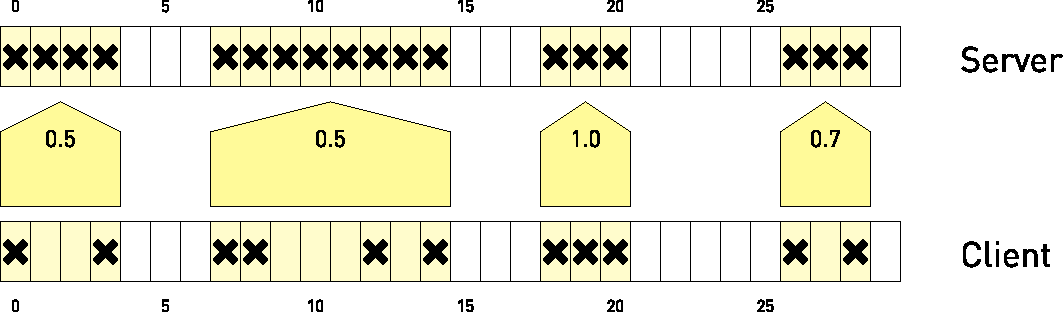
\includegraphics[width=0.85\textwidth]{figures/zusammenfassung_der_slots.pdf}
  \caption{Zusammenfassen von Slot-Bereichen zur �bertragung\label{zusammenfassung_der_slots}}
\end{figure}
Am effizientesten arbeitet dieser Ansatz wenn der Incore-Buffer anfangs noch leer ist da die Slots-Indices aufeinanderfolgend herausgegeben werden und die entsprechenden Speicherbereiche damit an einem St�ck auf den Server transferiert werden k�nnen. Das Zusammenfassen der Slots kann in einem Thread ausgelagert werden damit sich der entstehende Zeitaufwand nicht auf die Bildrate auswirkt. \\
\newpage

\newpage
\chapter{Ergebnisse und Diskussion}

\begin{figure}[position=h]
  \centering
  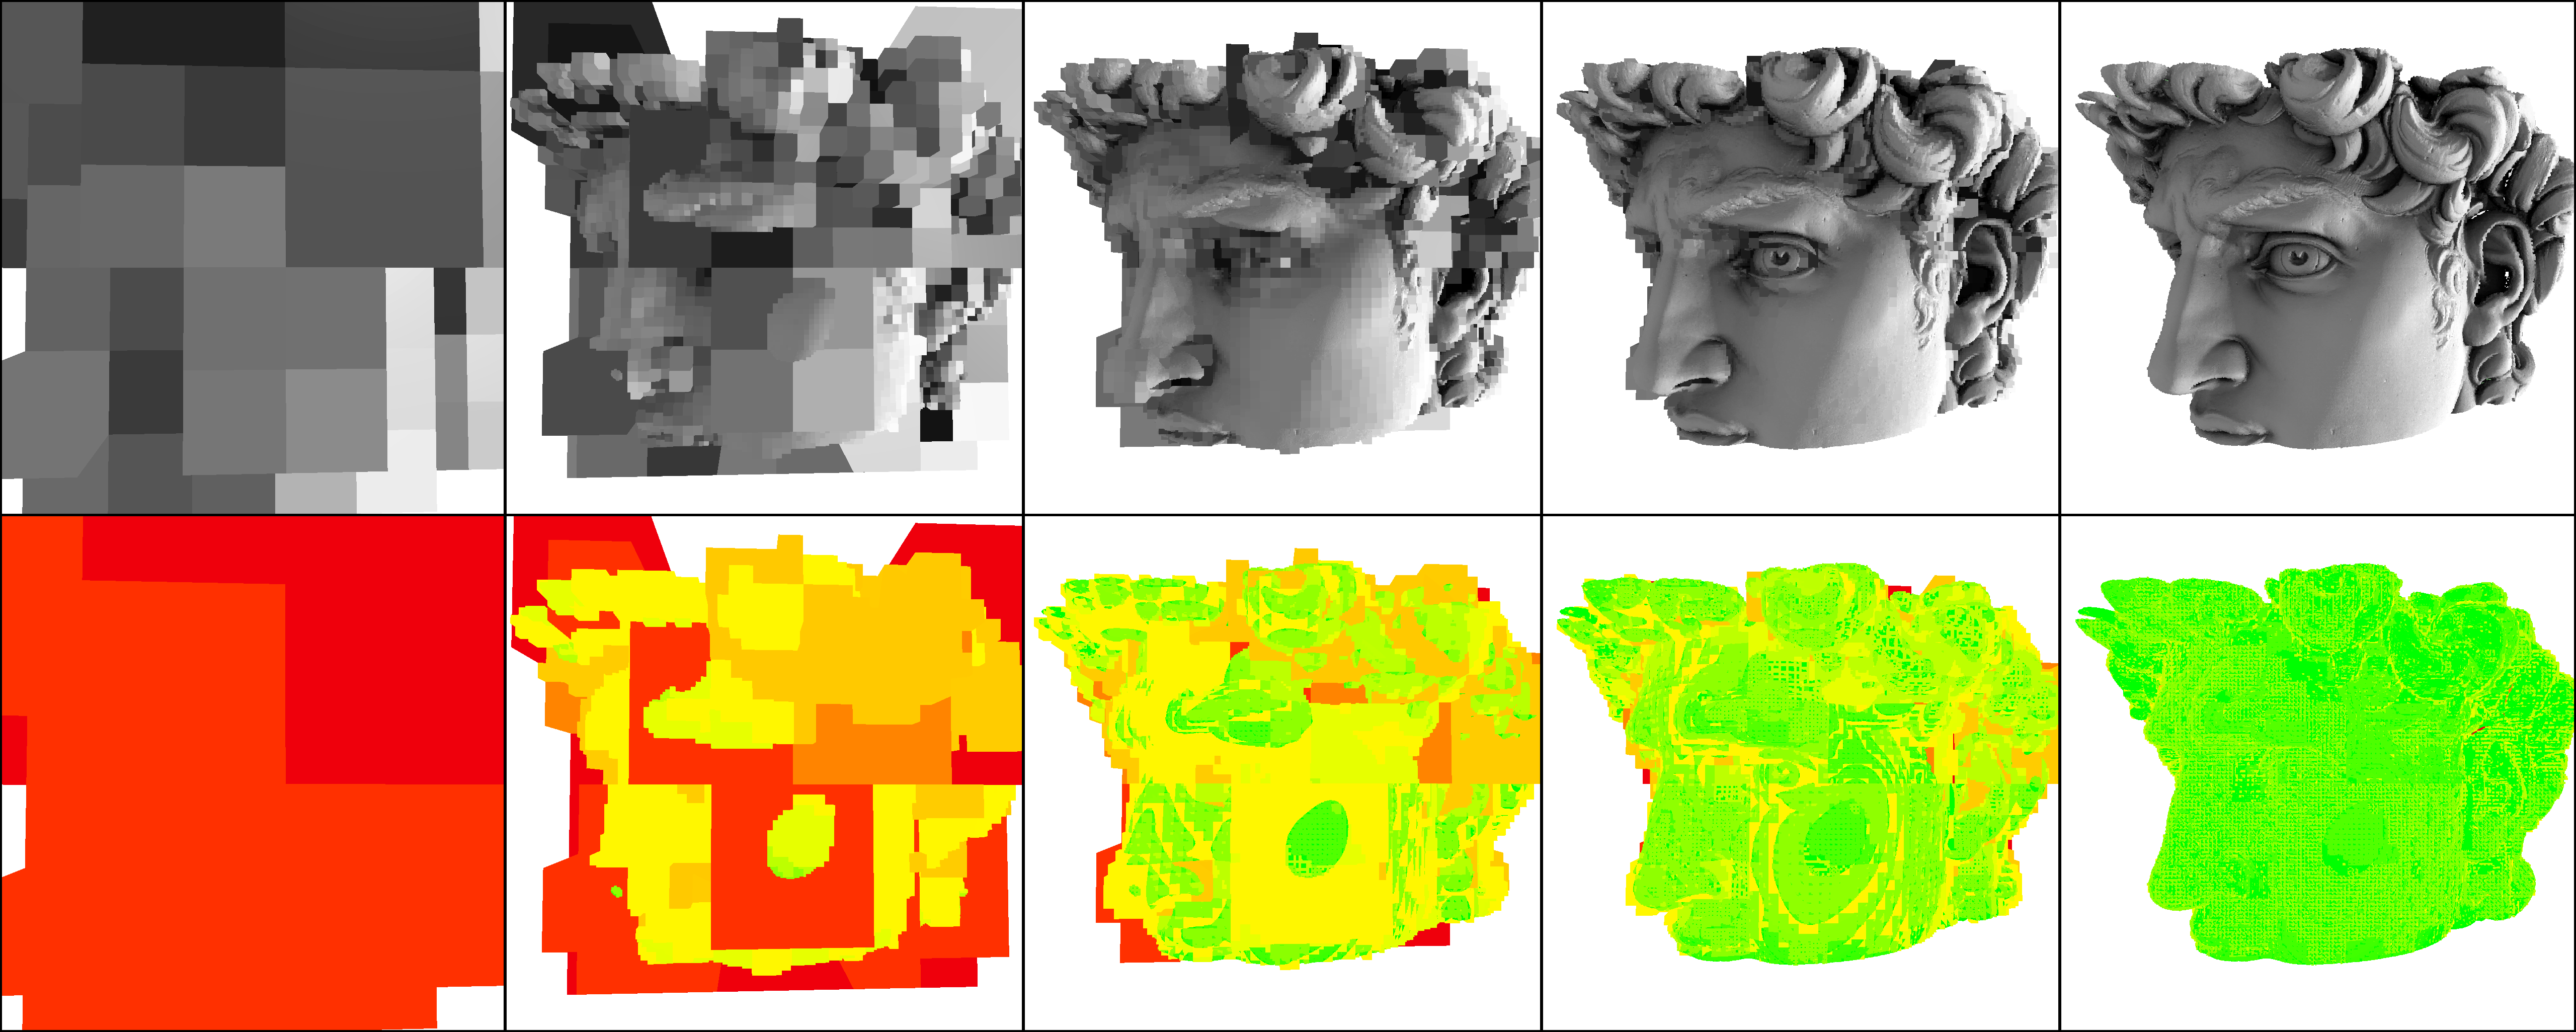
\includegraphics[width=1.0\textwidth]{figures/progressive_refinement.png}
  \caption{Verfeinerung in 5 aufeinander folgenden Schritten \label{progressive_refinement}}
\end{figure}

\section{�berblick}
\section{Verwendete Testszenen}
 

Zum Testen des Out-of-Core Systems wurden SVO-Strukturen f�r drei unterschiedliche Geometrien generiert (siehe Tabelle ...). 
Aus jeder Geometrie wurden zwei verschiedene SVO-Strukturen erstellt. Beide haben jeweils die selbe minimale Tiefe, aber eine unterschiedliche Treelet Gr��e. Die Tiefe betrug jeweils 12 bei Treelet Gr��en von 1kb und 4kb. Durch die Verkleinerung der Treelets bei gleicher minimaler SVO-Tiefe entstehen mehr Treelets und damit eine gr��erer Aufwand bei der Verwaltung. Die beiden Varianten sollen im folgenden verglichen werden, um die Skalierbarkeit des Out-of-Core Systems nach zu vollziehen. In Tabelle ... wird gezeigt... .

\begin{table}
\centering
\begin{tabular}{ l  r  r }
  \hline
  \textbf{Name} & \textbf{Anzahl Dreiecke} & \textbf{Dateigr��e} \\
  \hline
  David face       & 52.5 Mio & 14.7 GB \\
  \hline
  xyzrgb statuette & 10.0 Mio & 270 MB \\
  \hline  
  Lucy             & 28.0 Mio & 757 MB  \\
  \hline
\end{tabular}

\caption{Verwendete Modelle}\label{verwendete_modelle}
\end{table}




\begin{table}
\centering
\begin{tabular}{ l  r  r  r  r  r }
  \hline
  \textbf{Name} &  & \textbf{Treelet Gr��e} & \textbf{Anzahl Treelets} & \textbf{Anzahl Knoten} & \textbf{Dateigr��e} \\
  \hline
  David face        & 1kb & 743.277 &  95.139.456  & 000000\\
                    & 4kb & 484.297 & 247.960.064  & 000000\\
  \hline
  xyzrgb statuette  & 1kb & 13      & 000000      & 000000 \\
                    & 4kb & 13      & 000000      & 000000 \\
  \hline  
  Lucy              & 1kb & 13      & 000000      & 000000 \\
                    & 4kb & 13      & 000000      & 000000 \\
  \hline
\end{tabular}

\caption{Verwendete Modelle}\label{verwendete_modelle}
\end{table}
 
 

\section{Laufzeitanalyse}
Zum Testen wurden die Zeiten f�r die einzelnen Verarbeitungsschritte des Out-of-Core Systems gemessen. W�hrend der Messung wurde die Bildsynthese deaktiviert, um ausschlie�lich den Einfluss der Anzahl der Treelets auf den Ver\-walt\-ungsaufwandes zu untersuchen. Der SVO wurde �ber einen Zeitraum von 60 Sekunden aus verschiedenen Perspektiven analysiert und verfeinert. Durch die kontinuierliche Ver�nderung der Perspektive muss das System permanent neue Teile des Octrees anfordern, w�hrend es andere verwerfen muss. Damit bei der Verfeinerung auch Treelets in hohen Octree Tiefen angefordert werden, wird zum testen eine Kamerafahrt verwendet die ein Ma� an Koh�renz zwischen den Perspektiven zu gew�hrleisten.

\begin{figure}[position=h]
  \centering
  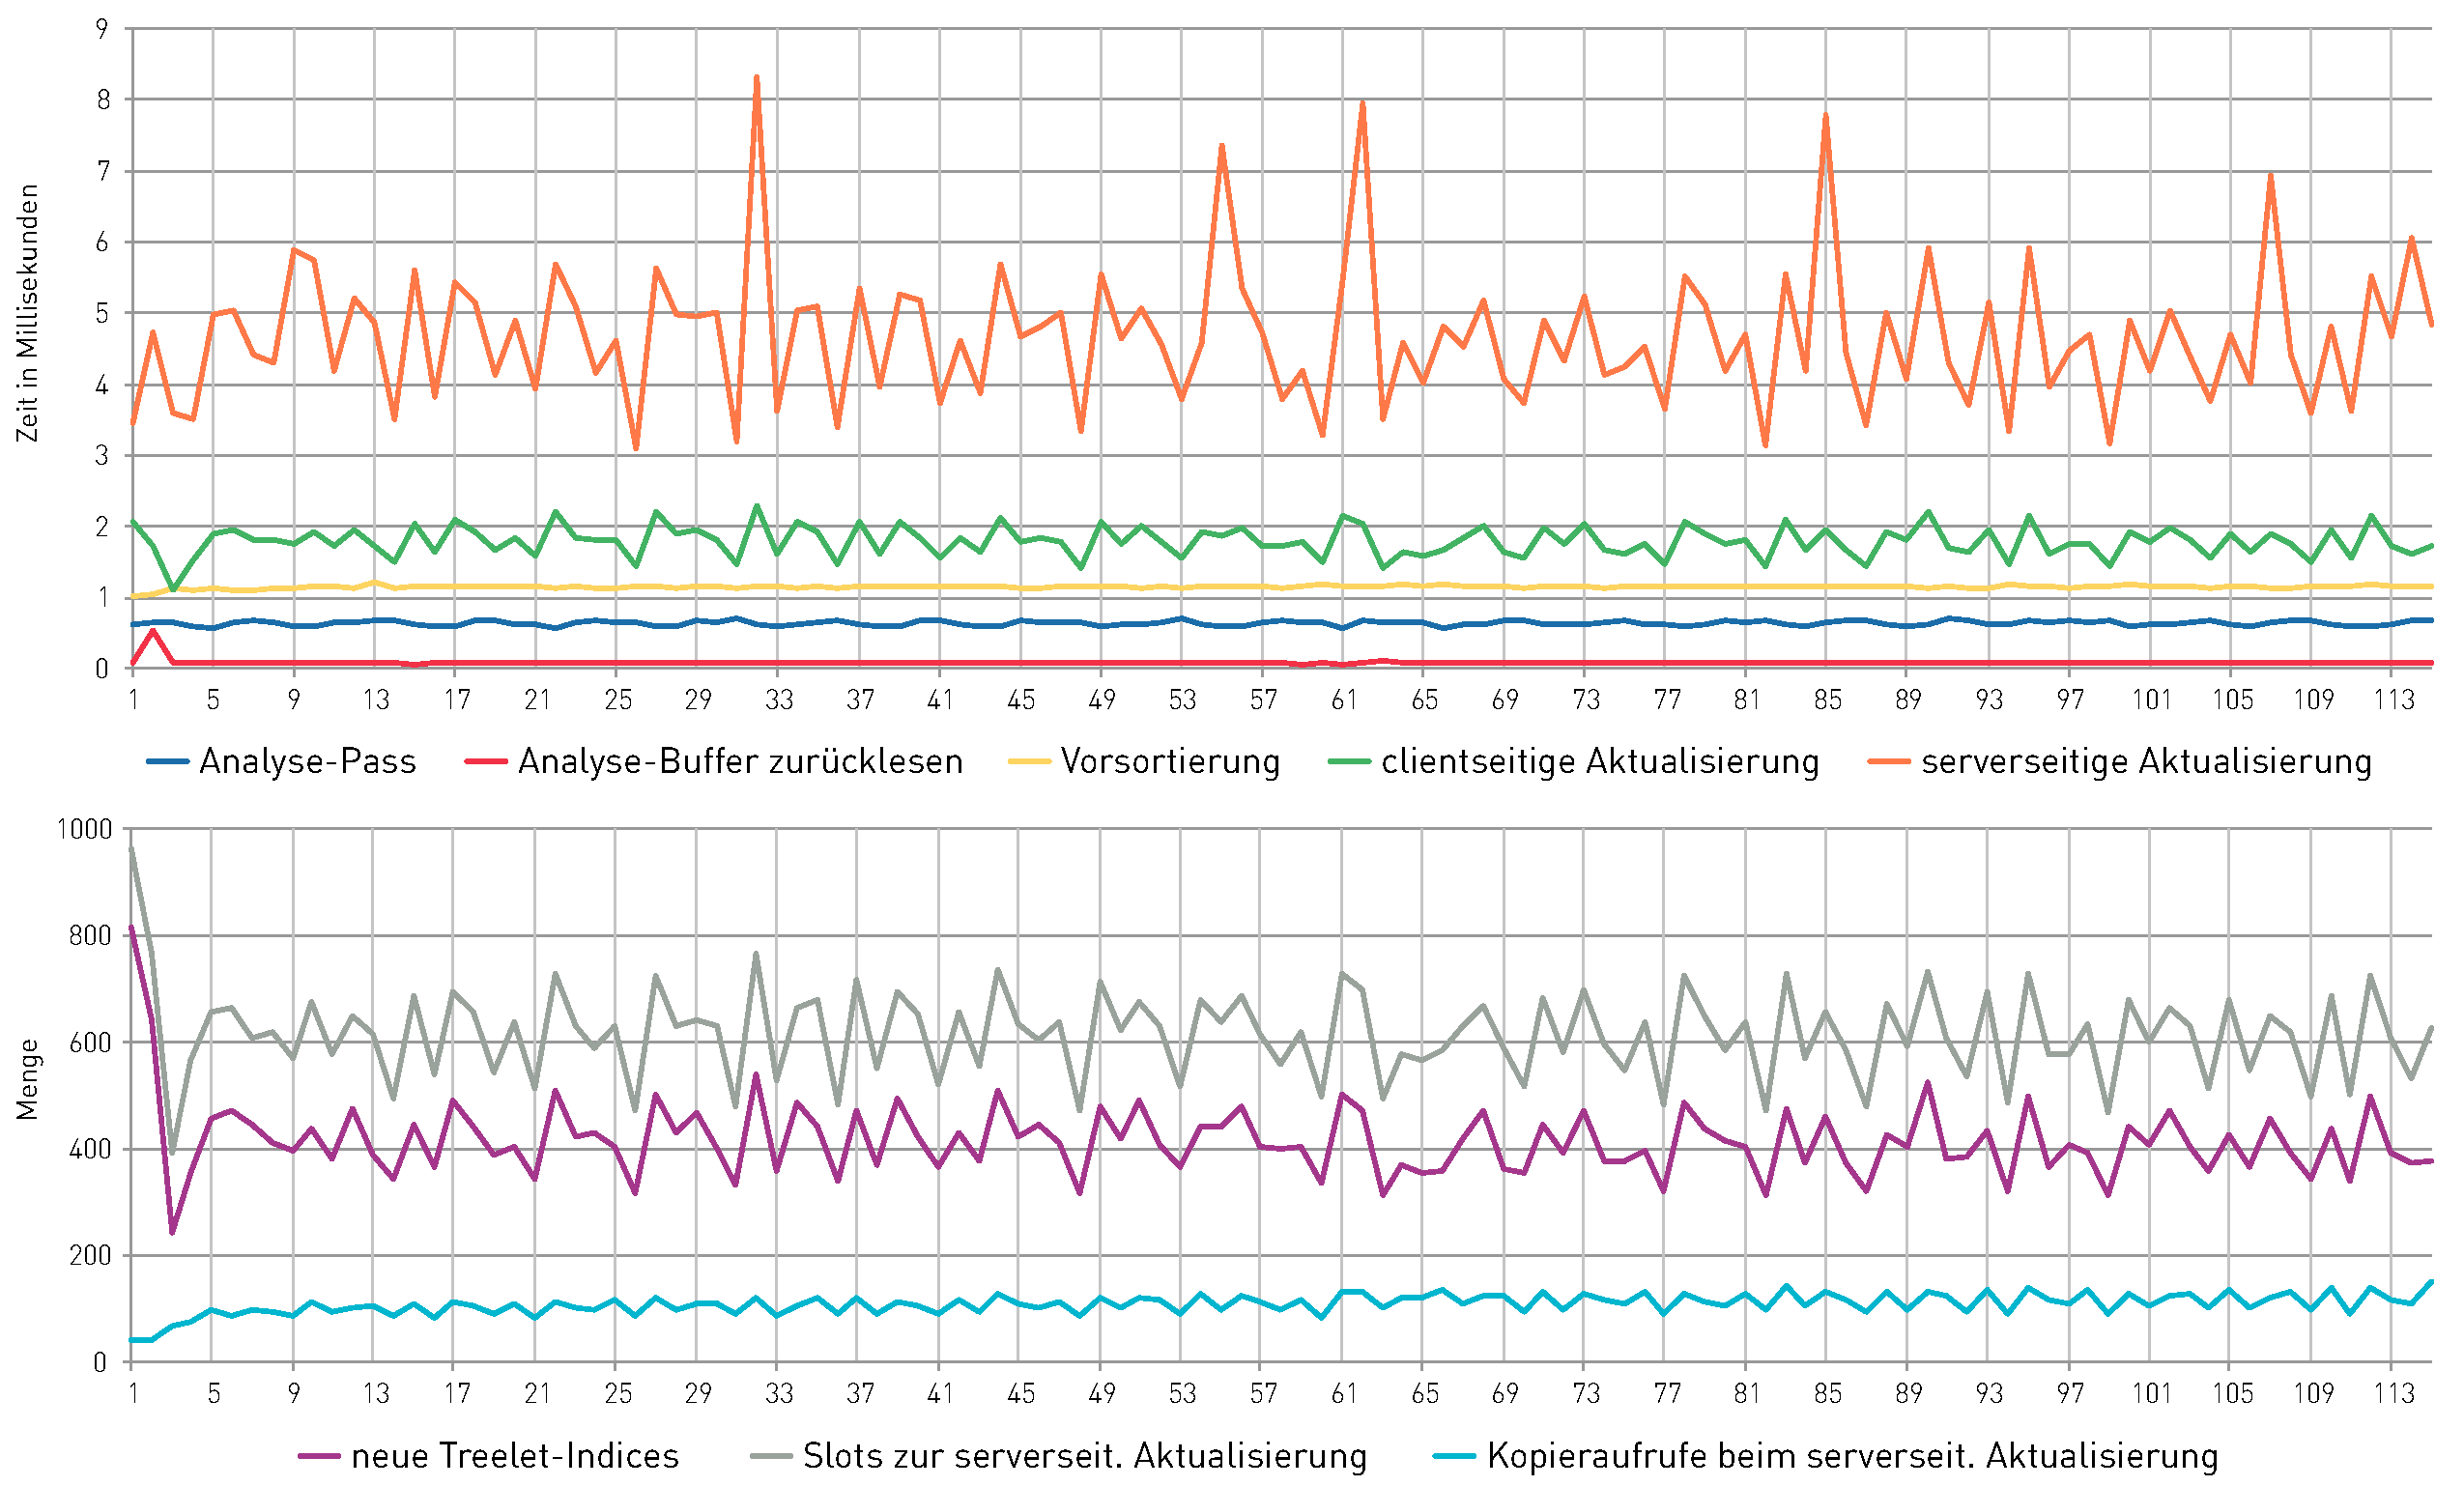
\includegraphics[width=1.0\textwidth]{figures/lucy_s4_D13_timeseries.pdf}
  \caption{Systemzeiten und Arbeit f�r Model lucy mit 4 kb Treelets\label{lucy_s4_D13_timeseries}}
\end{figure}

\begin{figure}[position=h]
  \centering
  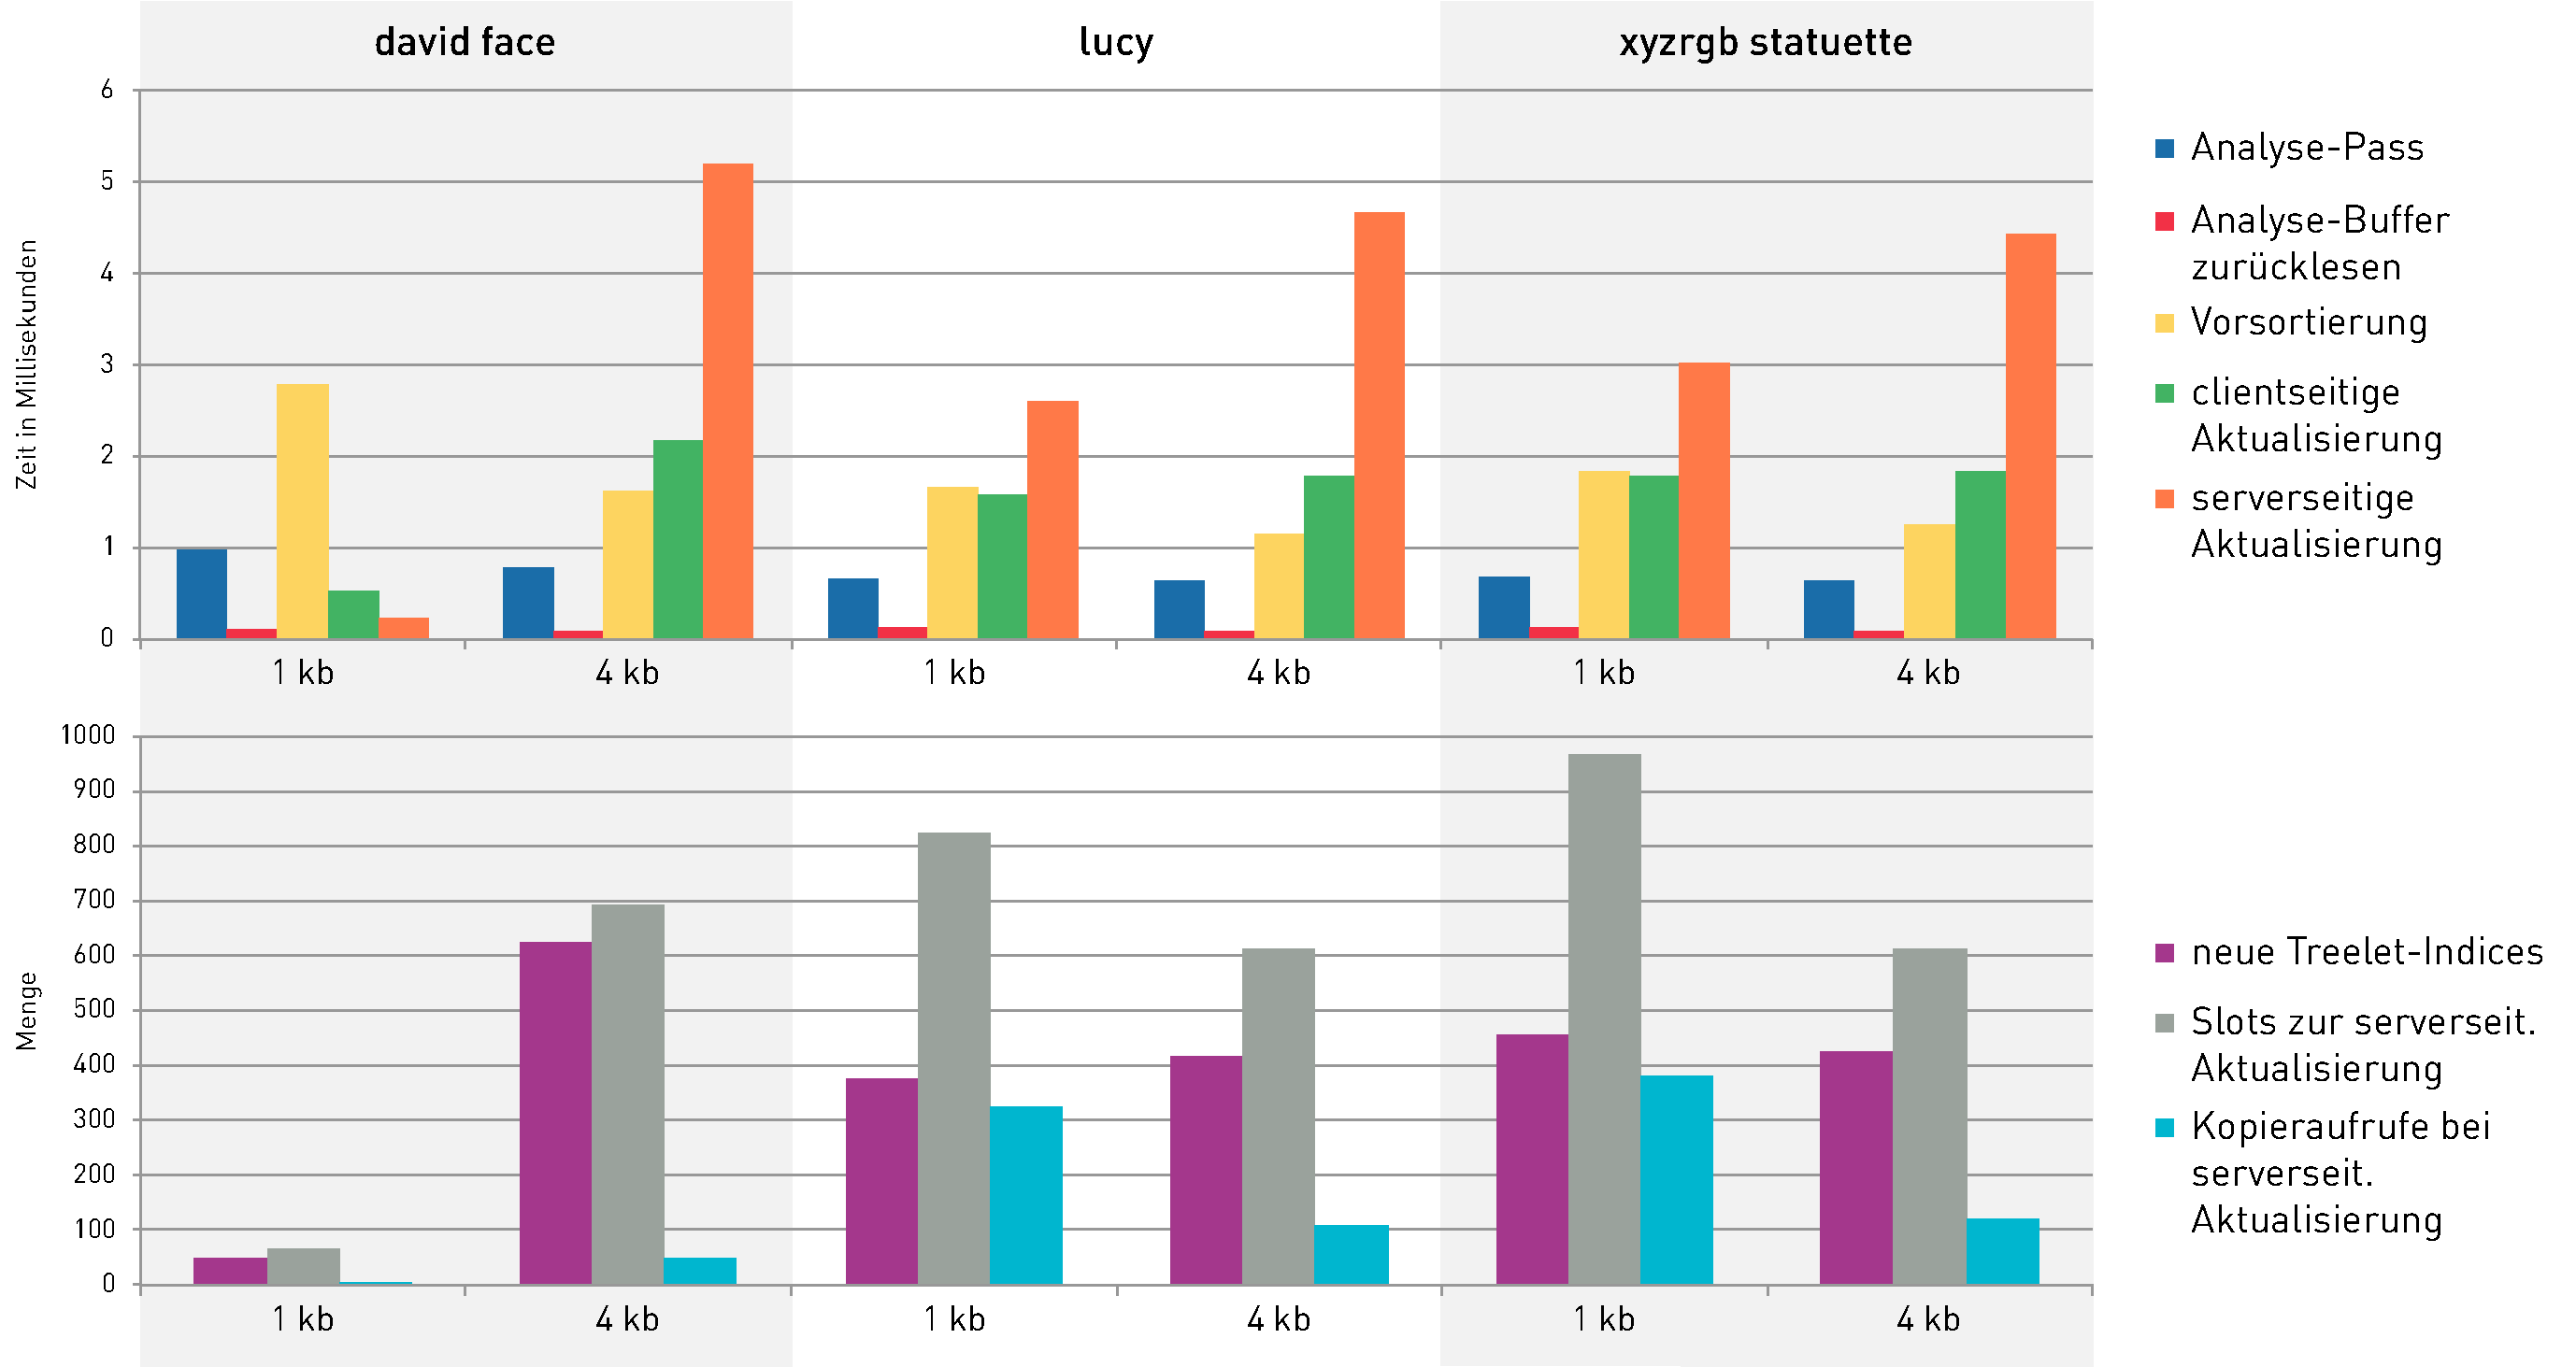
\includegraphics[width=1.0\textwidth]{figures/david_lucy_xyzrgb_s1_vs_24_D13.pdf}
  \caption{Gegen�berstellung unterschiedleichen Treelet-Gr��en\label{david_lucy_xyzrgb_s1_vs_24_D13}}
\end{figure}

\begin{figure}[position=h]
  \centering
  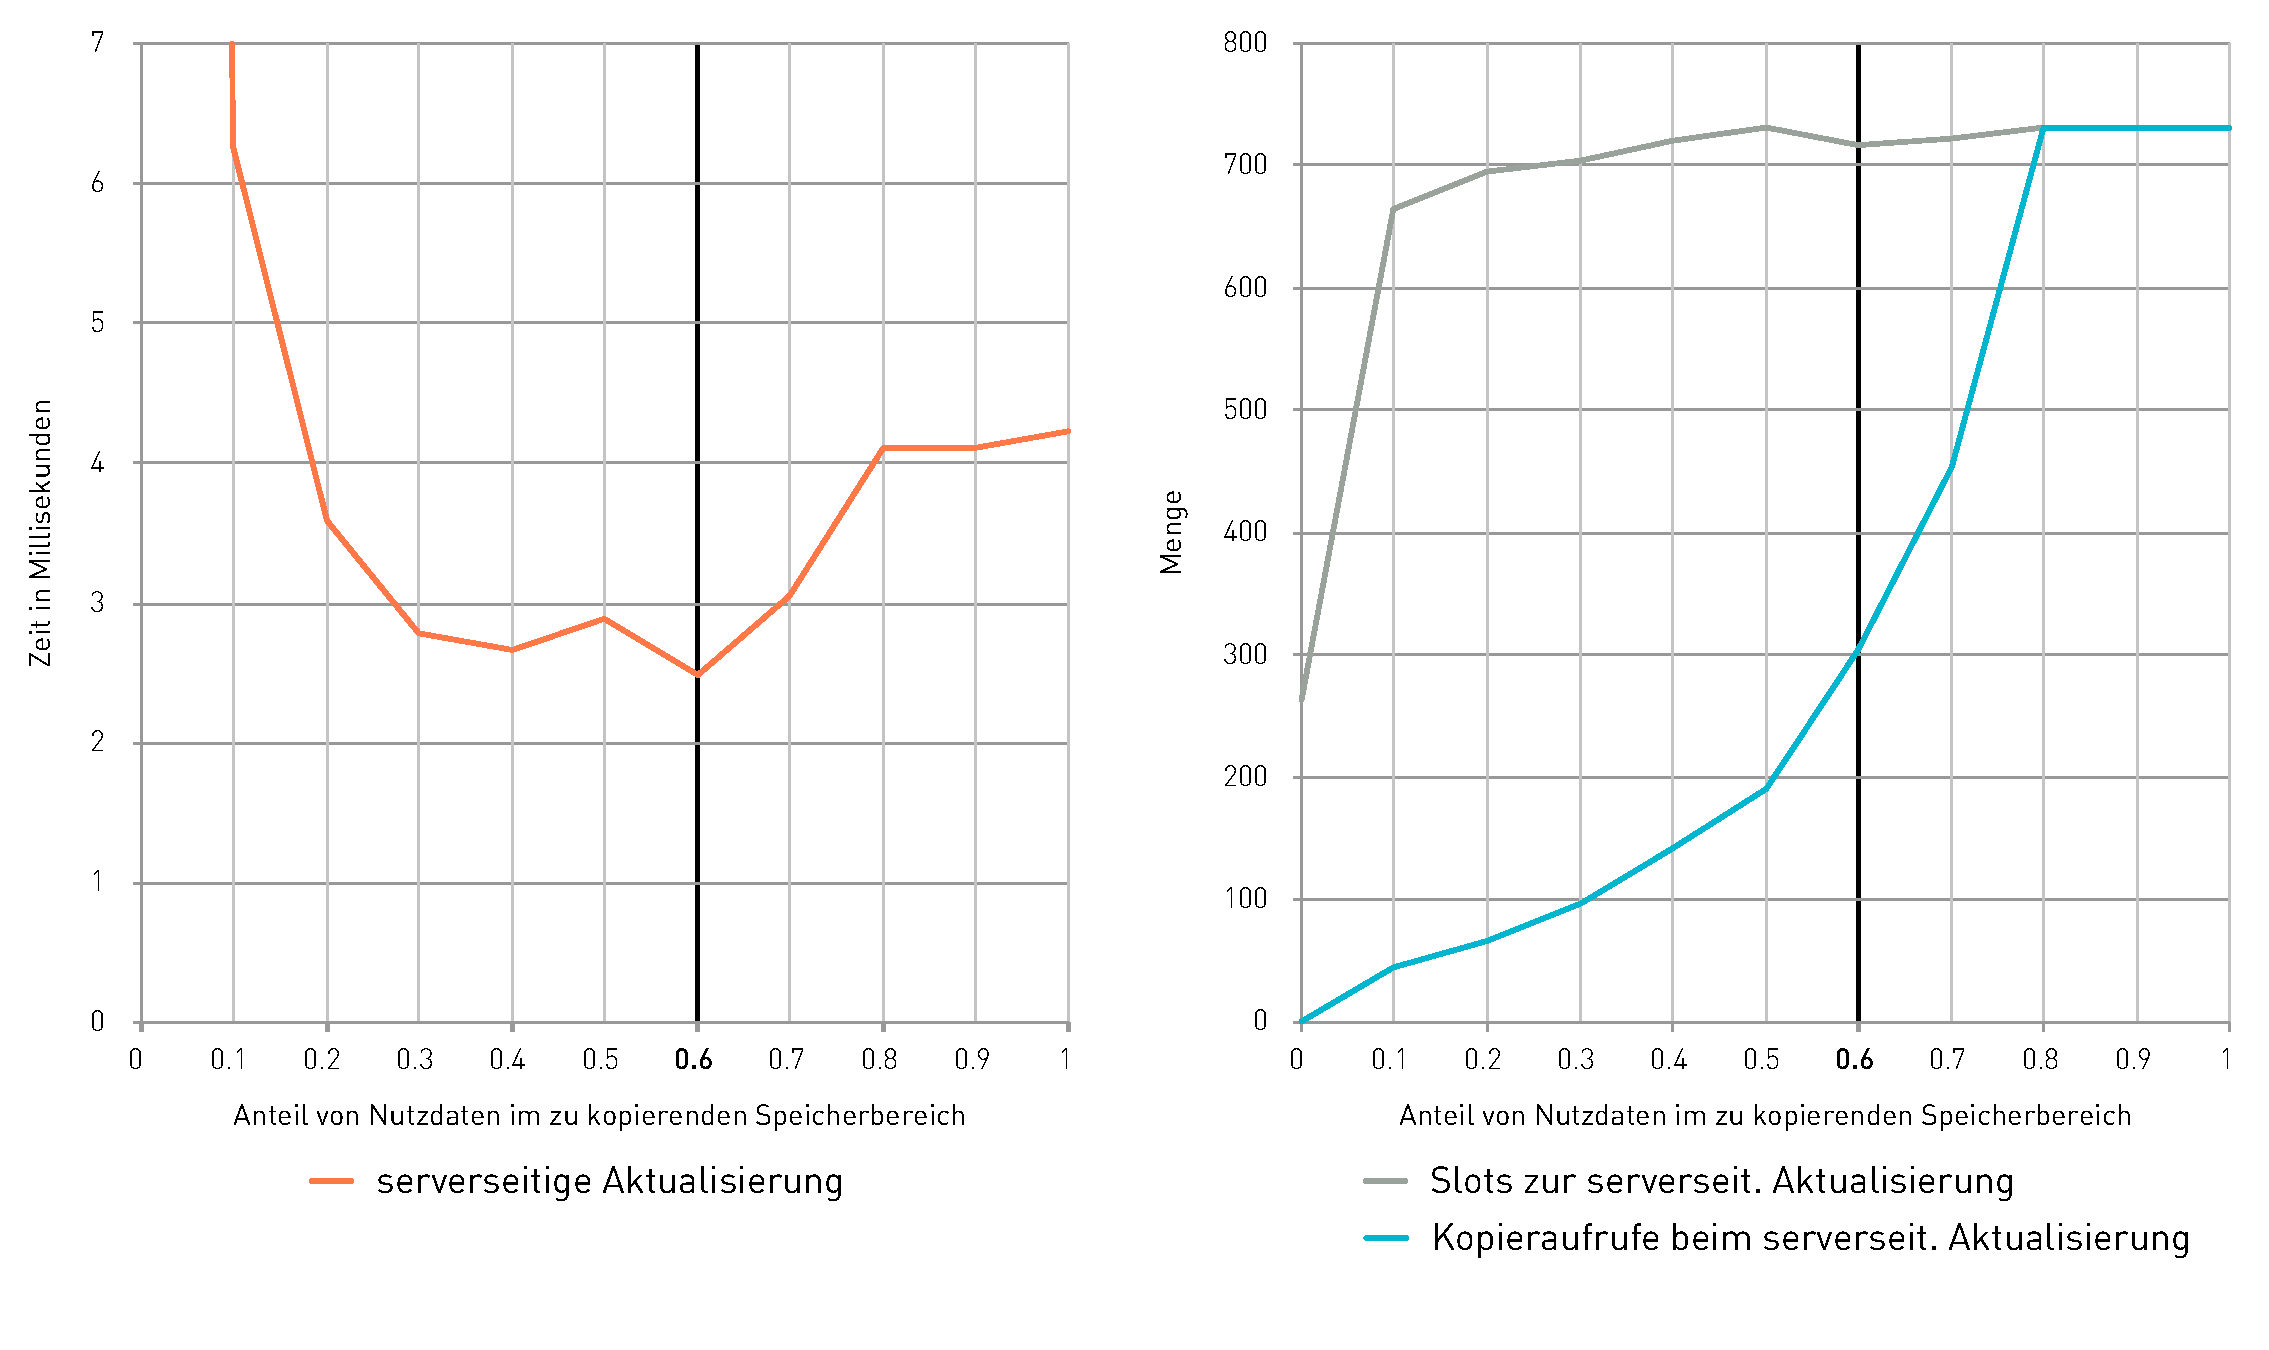
\includegraphics[width=1.0\textwidth]{figures/ratio_0-1.pdf}
  \caption{�fm�AFJa�FOJ\label{ratio_0-1}}
\end{figure}


\section{Einschr�nkungen und Verbesserungen}

\subsection{Serverseitige Aktualisierung}
Die in Abschnitt \ref{sec:serverseitige_aktualisierung} beschriebene Zusammenfassung der zu kopierenden Incore-Buffer-Slots wirkt sich deutlich auf die zum �bertragen der ge�nderten Speicherbereiche ben�tigte Zeit aus. Wie beschrieben arbeitet der Ansatz am besten wenn die zu transferierenden Speicherbereiche 
Mit steigender Fragmentierung des Incore-Buffers sinkt die Einsparung jedoch und schwankt stark. Bei einem vorgegebenen Verh�ltis zu aktualisierenden Slots von 20\% etwa schwankt die Einsparung zwischen 10\% bis 92\% und lag �ber einen Zeitraum von 60 Sekunden im Mittel bei etwa 43\%. Die hier examplarisch genannten Werte sind jedoch wenig aussagekr�ftig, da das Verhalten des Ansatzes nicht nur von der Anzahl der Slots, der Gr��e und dem Fragmentierungsgrad des Incore-Buffers abh�ngt, sondern auch von der Geometrie und der Kameraposition �ber die Zeit. Eine Verbesserung zum einzelnen Kopieren der Slots ist jedoch erkennbar.

\subsection{Verwendung von OpenGL Texturen als Buffer}
...

\newpage
\chapter{Zusammenfassung und Ausblick}


\section{Zusammenfassung}

Der Schwerpunkt der vorliegende Arbeit liegt auf...

In der vorliegende Arbeit wurde ein Out-of-Core Ansatz zur Darstellung von gro�en Sparse Voxel Octree Strukturen entwickelt. Diesem liegt eine Segmentierung der Octree Daten durch Aufteilung in Unterb�ume gleicher Gr��e zugrunde. Zur Erstellung von Inhalten wurde ein generalisiertes System zur SVO Erstellung implementiert. 



Die daraus entstanden Applikation kann ... , weil ... . OpenCL. Weiterin wurde ein ... .


Die Tests haben gezeigt ... 


\section{Ausblick}


\newpage
\addcontentsline{toc}{chapter}{Quellen}
\addcontentsline{toc}{section}{Literaturverzeichnis}
\bibliographystyle{jas99}
\bibliography{literatur}
\newpage

\chapter{Glossar}


\textbf{Aliasing}\\
Beim Abtasten von Daten mit zu geringer Abtastfrequenz entstehende Fehler. Diese f�hren in Dar\-stel\-lungen zu Mustern und Bildartefakten, die nicht in den Originaldaten enthalten sind. 
\\
\\
\textbf{Ambient Occlusion}\\
Eine Shading-Methode zur Simulation globaler Beleuchtungsdaten. Dabei wird ein Ma� der Verdeckung eines Teils der Daten durch benachbarte Bereiche ermittelt und auf die Beleuchtungdaten angewendet. 
\\
\\
\textbf{Antialiasing}\\
Techniken zur Minimierung von Aliasing.
\\
\\
\textbf{Bounding Box}\\
Ein Quader oder W�rfel, der zur Optimierung von Berechnungen komplexere, in diesem Volumen ent\-haltene Daten repr�sentiert.
\\
\\
\textbf{Culling}\\
Ein Verfahren, bei dem mit Hilfe von Sichtbarkeits- und Verdeckungsinformationen eine Reduzierung der zur Bilderzeugung zu verarbeitenden Daten erreicht werden kann. 
\\
\\
\textbf{GPGPU} (General-purpose computing on graphics processing units)\\
Bezeichnet die Verwendung eines Grafikprozessors zur L�sung auch andere algorithmische Probleme.
\\
\\
\textbf{Mipmaps}\\
Eine LOD-Technik f�r Texturen, die zur Vermeidung von Aliasing-Artefakten verwendet wird. Eine Mipmap besteht aus einer hierarchischen Anordnung von unterschiedlich aufgel�sten Repr�sentationen der Ausgangsdaten. W�hrend der Bilderzeugung werden diejenigen Repr�sentationen ausgew�hlt, die der Bildaufl�sung am besten entsprechen.  
\\
\\
\textbf{Popping-Artefakt}\\
Eine pl�tzliche und deutlich sichtbare �nderung der Darstellung. Oft entstehen diese Artefakte aufgrund eines �bergangslosen Wechsels der, f�r die Darstellung verwendeten Detailstufen. 
\\
\\
\textbf{Raycasting}\\
Eine Methode zur Visualisierung von Daten. Dabei wird pro darzustellendem Bildpunkt der Weg von mindestens einem Strahl durch die r�umlichen Daten berechnet. Dabei werden beispielsweise Farb- und Beleuchtungswerte ermittelt.  
\\
\\
\textbf{Speicherkoh�renz}\\
Eine Eigenschaft von Speicherzugriffen, die sich aus der Entfernung zwischen aufeinanderfolgenden Zugriffen ergibt. F�r Zugriffe auf benachbare Speicherregionen, ist die Speicherkoh�renz hoch. Operationen mit hoher Speicherkoh�renz lassen sich oft effizienter ausf�hren, als solche mit niedriger Speicherkoh�renz.
\\
\\
\textbf{UV-Koordinaten}\\
Eine Fl�chenkoordinate, die zum Abbilden von Texturdaten auf 3D-Objekte verwendet wird. 
\\
\\
\textbf{Client-Server-Architektur}\\
Beschreibt ein aus zwei Subsystemen bestehendes System. Der Server stellt dabei Dienste zur Verf�gung, die vom Client angefordert werden.
\end{document}